\documentclass[conference]{IEEEtran}
\usepackage{graphicx}
\usepackage{amsmath}
\usepackage{amssymb}
\usepackage{hyperref}
\usepackage{booktabs}
\usepackage{multirow}
\usepackage{color}
\usepackage{float}
\usepackage{caption}
\usepackage{subcaption}
\usepackage{enumerate}
\usepackage{listings}

\hypersetup{
    colorlinks=true,
    linkcolor=blue,
    filecolor=magenta,
    urlcolor=cyan,
    citecolor=blue
}

\begin{document}

\title{The Impact of AI Coding Tools on Developer Productivity and Perception: A Data Mining Analysis}

\author{
\IEEEauthorblockN{Data Warehousing and Mining Project}
\IEEEauthorblockA{Department of Computer Science\\
University Name\\
Location\\
email@domain.edu}
}

\maketitle

\begin{abstract}
This research examines the usage patterns, impacts, and perceptions of artificial intelligence (AI) coding tools among software developers, data scientists, students, and researchers. Through analysis of survey data from 97 professionals with diverse backgrounds, experience levels, and roles, we uncover key insights into how AI is transforming software development practices. Our findings reveal significant patterns in adoption rates, perceived benefits, concerns, and overall impact on productivity and creativity across different demographic segments. Results indicate that while AI tools substantially enhance productivity for experienced professionals, concerns about dependency, job replacement, and bias persist, particularly among specific demographic groups. This research provides valuable insights for AI tool developers, organizations adopting these technologies, and individual practitioners navigating the evolving landscape of AI-assisted software development.
\end{abstract}

\begin{IEEEkeywords}
AI coding tools, software development, developer productivity, data mining, ChatGPT, GitHub Copilot, trust in AI
\end{IEEEkeywords}

\section{Introduction}
The rise of AI-powered coding tools such as GitHub Copilot, ChatGPT, Tabnine, and Codeium has significantly transformed the landscape of software development. These tools leverage machine learning models to assist developers by providing code suggestions, enhancing documentation, facilitating debugging, and generating complete code segments. Despite their growing popularity, comprehensive studies examining their usage patterns and impact across different professional roles and experience levels remain limited.

This research aims to bridge this gap by analyzing a diverse dataset of professionals who use AI coding tools. We employ data mining techniques to uncover patterns in adoption, usage frequency, perceived benefits, and concerns. Additionally, we examine how different demographic factors influence perceptions and utilization of these tools, providing insights into the evolving relationship between AI and software development.

The key research questions addressed in this study include:
\begin{enumerate}
    \item How do adoption rates and usage patterns of AI coding tools vary across different demographic segments and professional roles?
    \item What impact do these tools have on developers' productivity, code quality, and creativity?
    \item How does experience level influence trust in and concerns about AI-generated code?
    \item What are the most common concerns regarding AI coding tools, and how do these vary by professional context?
    \item What future capabilities are most desired by different segments of the development community?
\end{enumerate}

By addressing these questions, this study contributes to our understanding of how AI is reshaping software development practices and provides guidance for tool developers, organizations, and individual practitioners navigating this technological transition.

\section{Methodology}
\subsection{Data Collection}
The dataset comprises survey responses from 97 participants including software developers, data scientists, researchers, and students with varying levels of experience and educational backgrounds. The survey collected information on:
\begin{itemize}
    \item Demographic information (age, education, role, coding experience)
    \item Programming language preferences
    \item AI tool usage patterns and frequency
    \item Perceived impact on coding speed and code quality
    \item Primary uses of AI coding tools
    \item Trust levels in AI-generated code
    \item Perceived impact on creativity
    \item Concerns about AI coding tools
    \item Perceptions regarding AI potentially replacing developers
    \item Desired improvements in AI tools
    \item Requested autonomous software capabilities
\end{itemize}

\subsection{Data Analysis Approach}
We employed descriptive statistics, frequency analysis, and cross-tabulation to identify patterns and relationships within the data. Visualization techniques including bar charts and heatmaps were used to represent distributions and correlations. The analysis focused on:

\begin{enumerate}
    \item Demographic distribution of AI tool adoption
    \item Relationship between experience level and AI tool usage/perception
    \item Impact of AI tools on different aspects of software development
    \item Common concerns and trust levels across professional roles
    \item Correlation between AI tool usage frequency and perceived benefits
    \item Future software capabilities desired by different professional groups
\end{enumerate}

Python was used for data analysis, with pandas for data manipulation, matplotlib and seaborn for visualization, and numpy for numerical operations. Cross-tabulation analyses were performed to identify relationships between categorical variables such as professional role and AI tool usage frequency.

\section{Results}
\subsection{Demographic Distribution}
Our survey sample consisted of 97 participants with diverse backgrounds. The age distribution showed a concentration in the 25-34 (27.8\%) and 35-44 (27.8\%) age brackets, followed by younger professionals aged 18-24 (23.7\%). Mid-to-late career professionals aged 45-54 represented 14.4\% of participants, while those 55 and older constituted 6.2\%.

\begin{figure}[H]
    \centering
    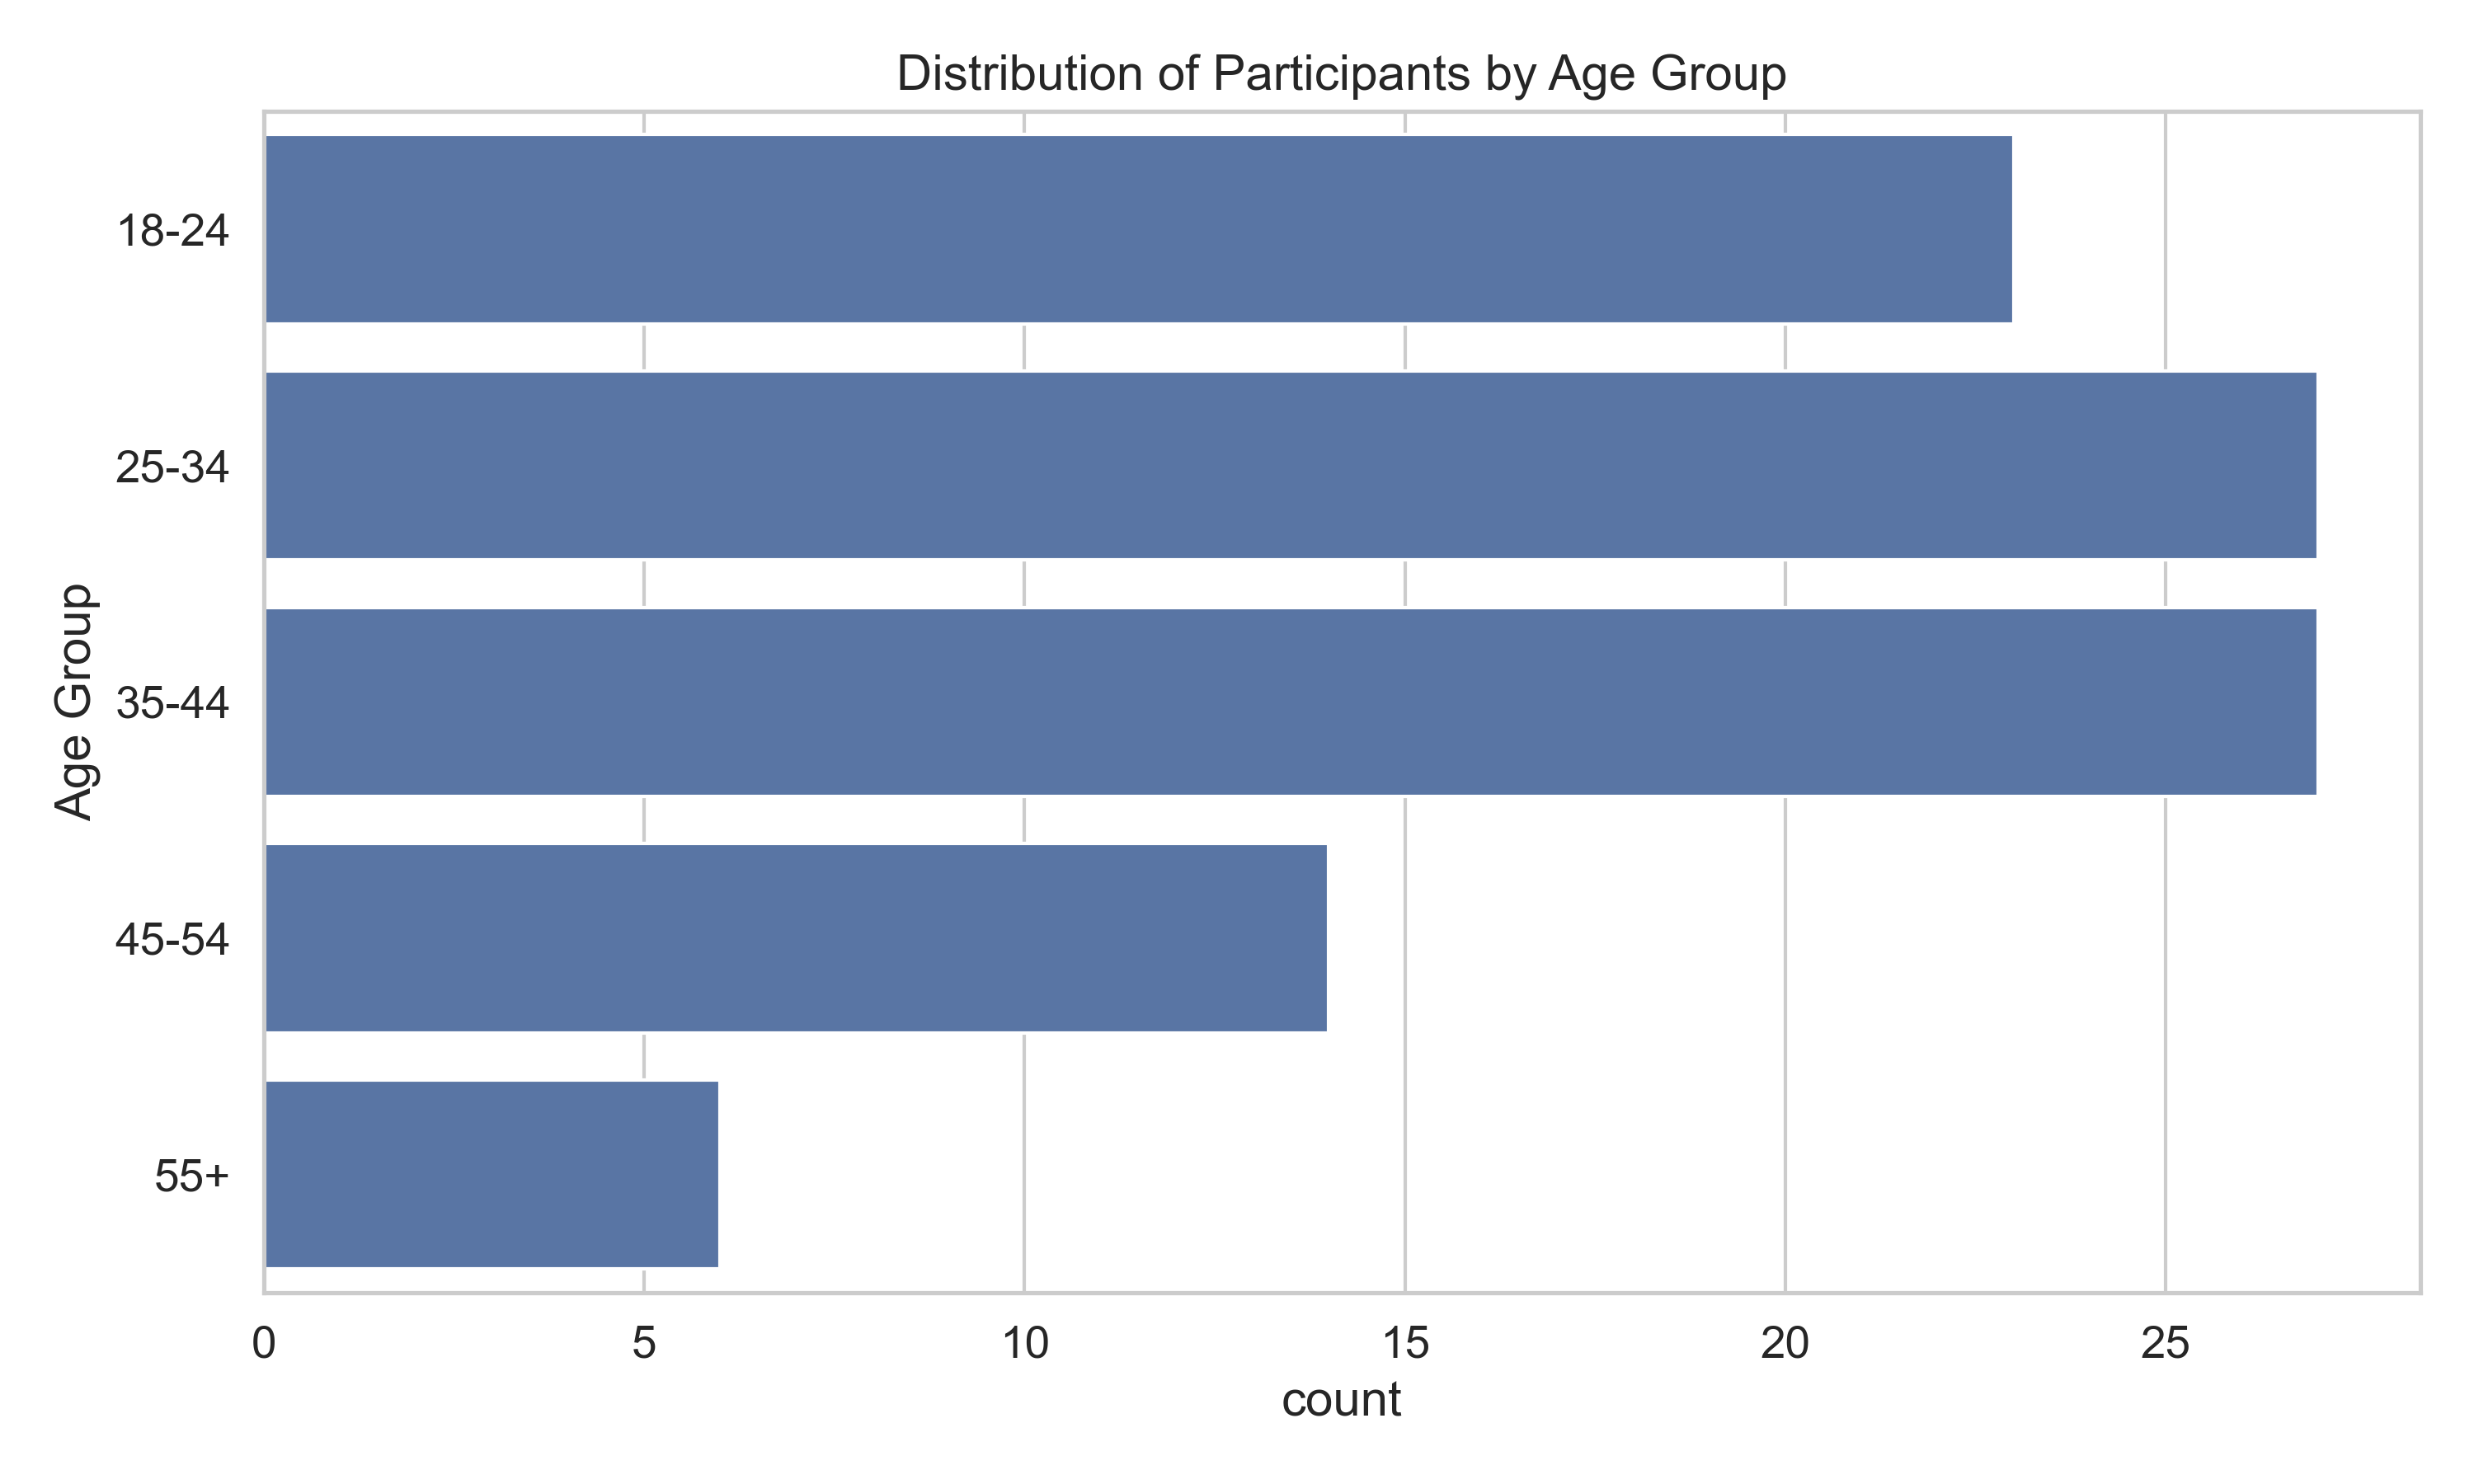
\includegraphics[width=0.8\linewidth]{final_research/age_distribution.png}
    \caption{Distribution of participants by age group}
    \label{fig:age_distribution}
\end{figure}

In terms of professional roles, Software Developers formed the largest group (28.9\%), followed by Students (23.7\%), Researchers (19.6\%), Data Scientists/ML Engineers (16.5\%), and Freelancers (11.3\%). This distribution provides a comprehensive view across the software development ecosystem.

\begin{figure}[H]
    \centering
    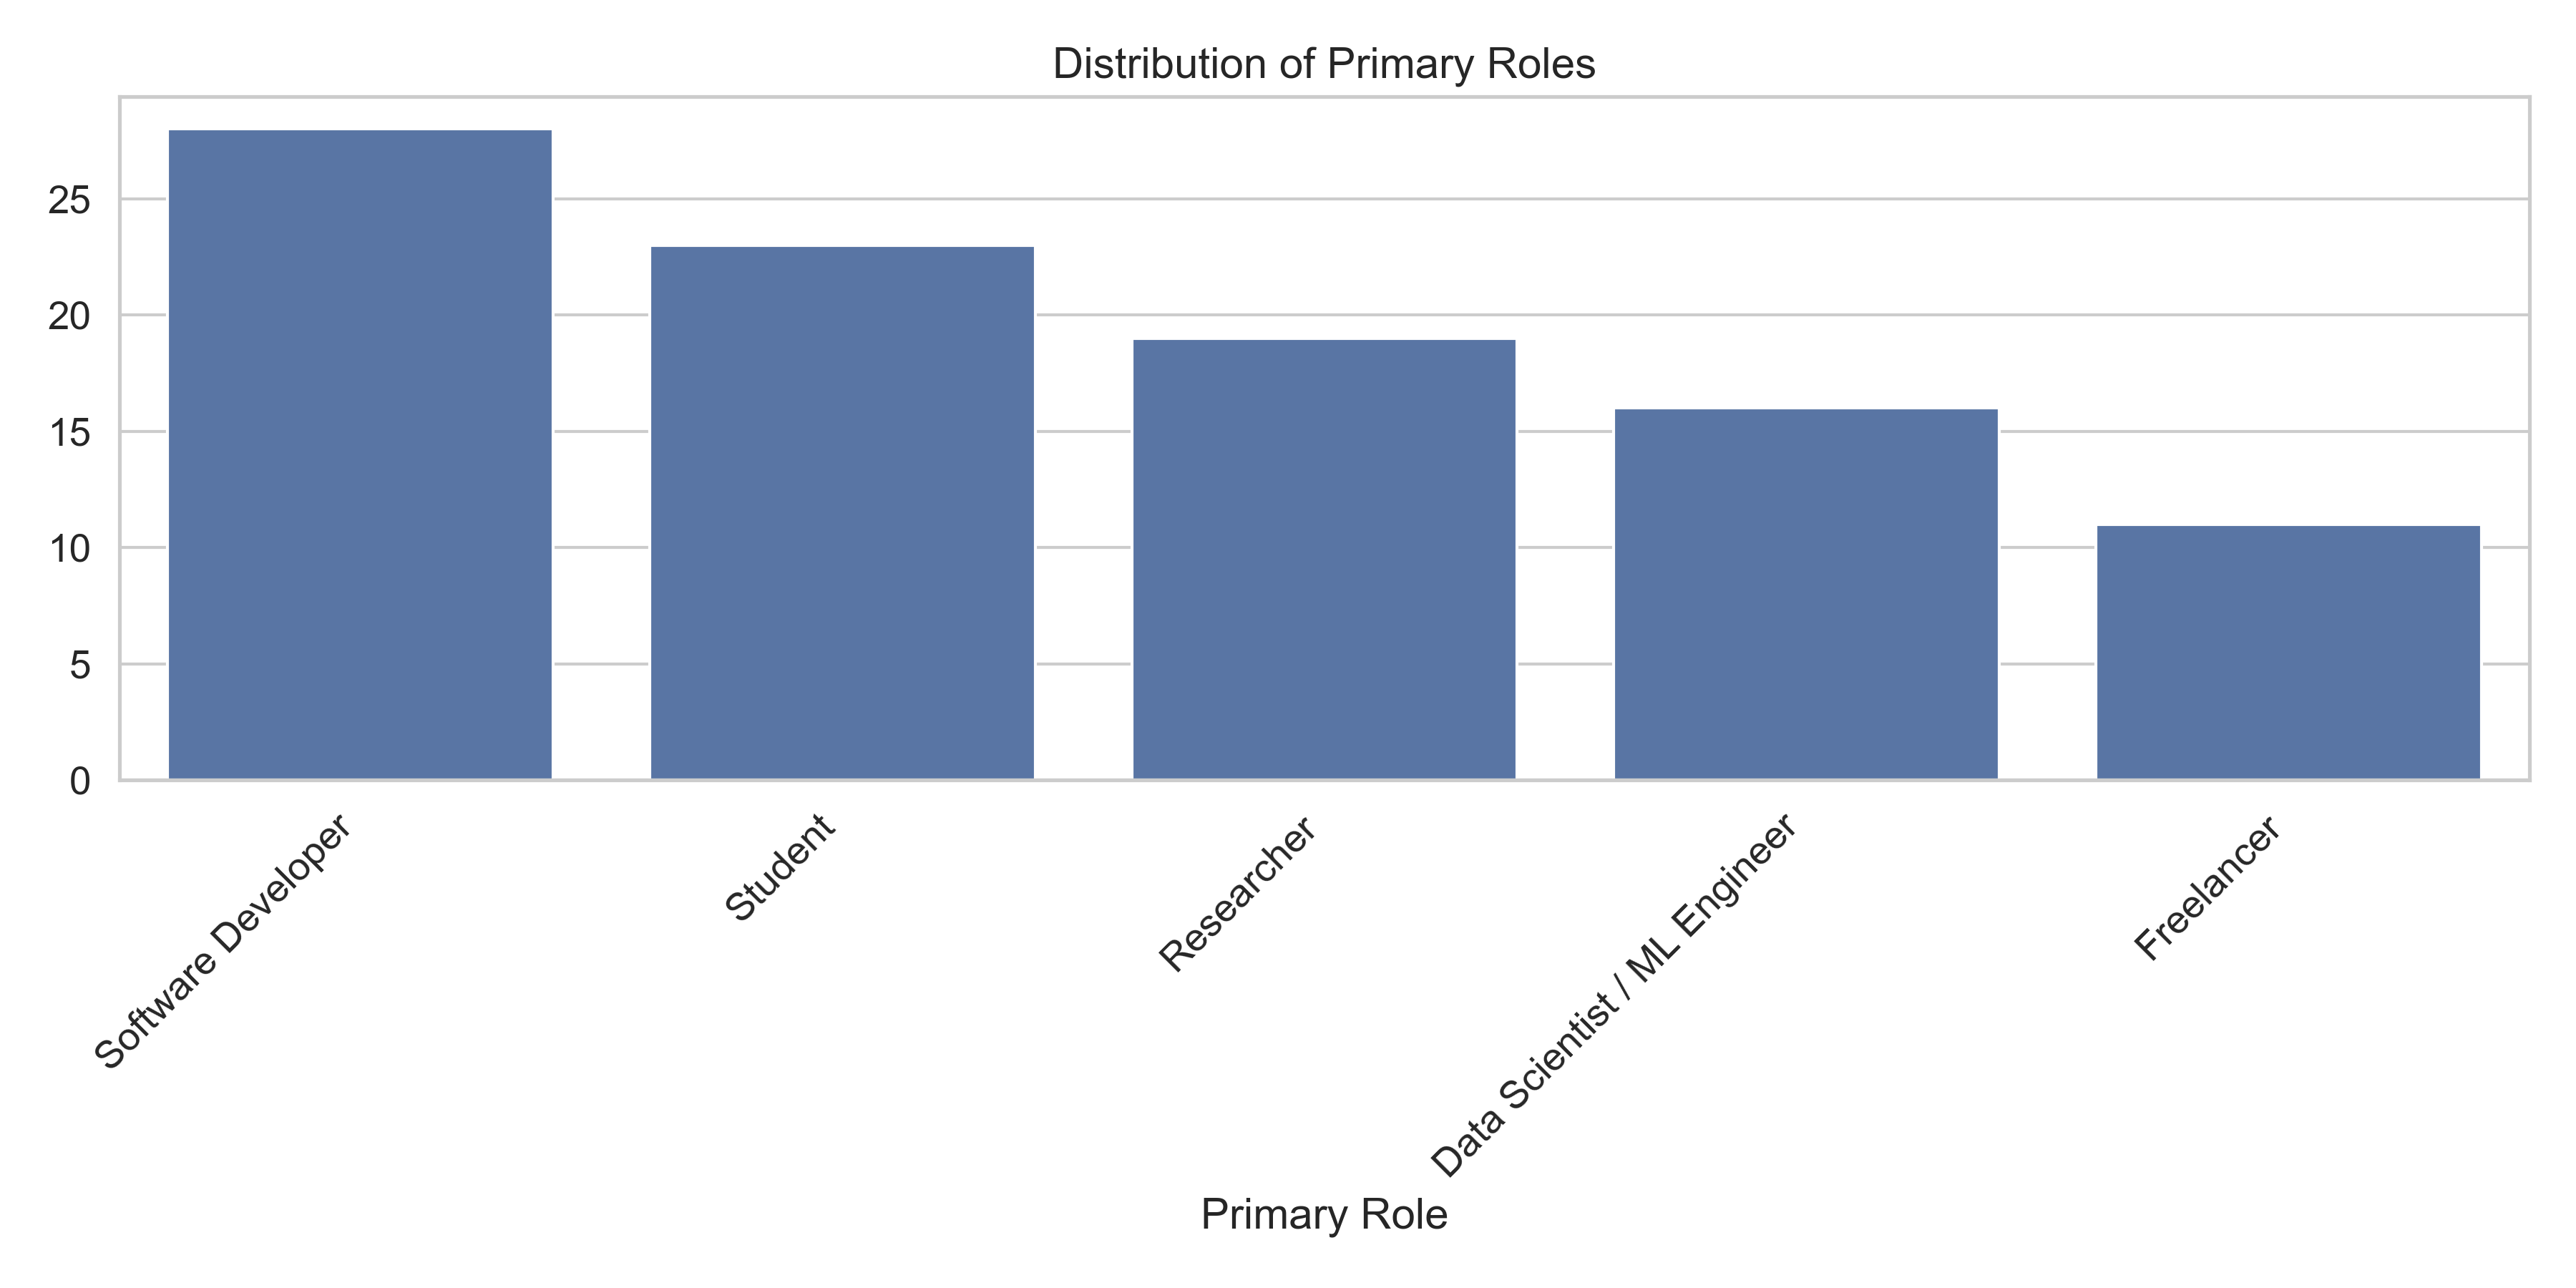
\includegraphics[width=0.8\linewidth]{final_research/role_distribution.png}
    \caption{Distribution of participants by primary role}
    \label{fig:role_distribution}
\end{figure}

Educational attainment was relatively high among participants, with 36.1\% holding Master's degrees, 32.0\% with Bachelor's degrees, and 19.6\% with Ph.D. degrees. High school graduates comprised 12.4\% of the sample, primarily represented in the student category.

Regarding coding experience, nearly half of the participants (48.5\%) had more than 7 years of experience, 27.8\% had 4-6 years, 13.4\% had 1-3 years, and 10.3\% had less than one year of coding experience. Python was the most commonly used programming language (40.2\%), followed by JavaScript (18.6\%), Java (11.3\%), and C++ (8.2\%).

\begin{figure}[H]
    \centering
    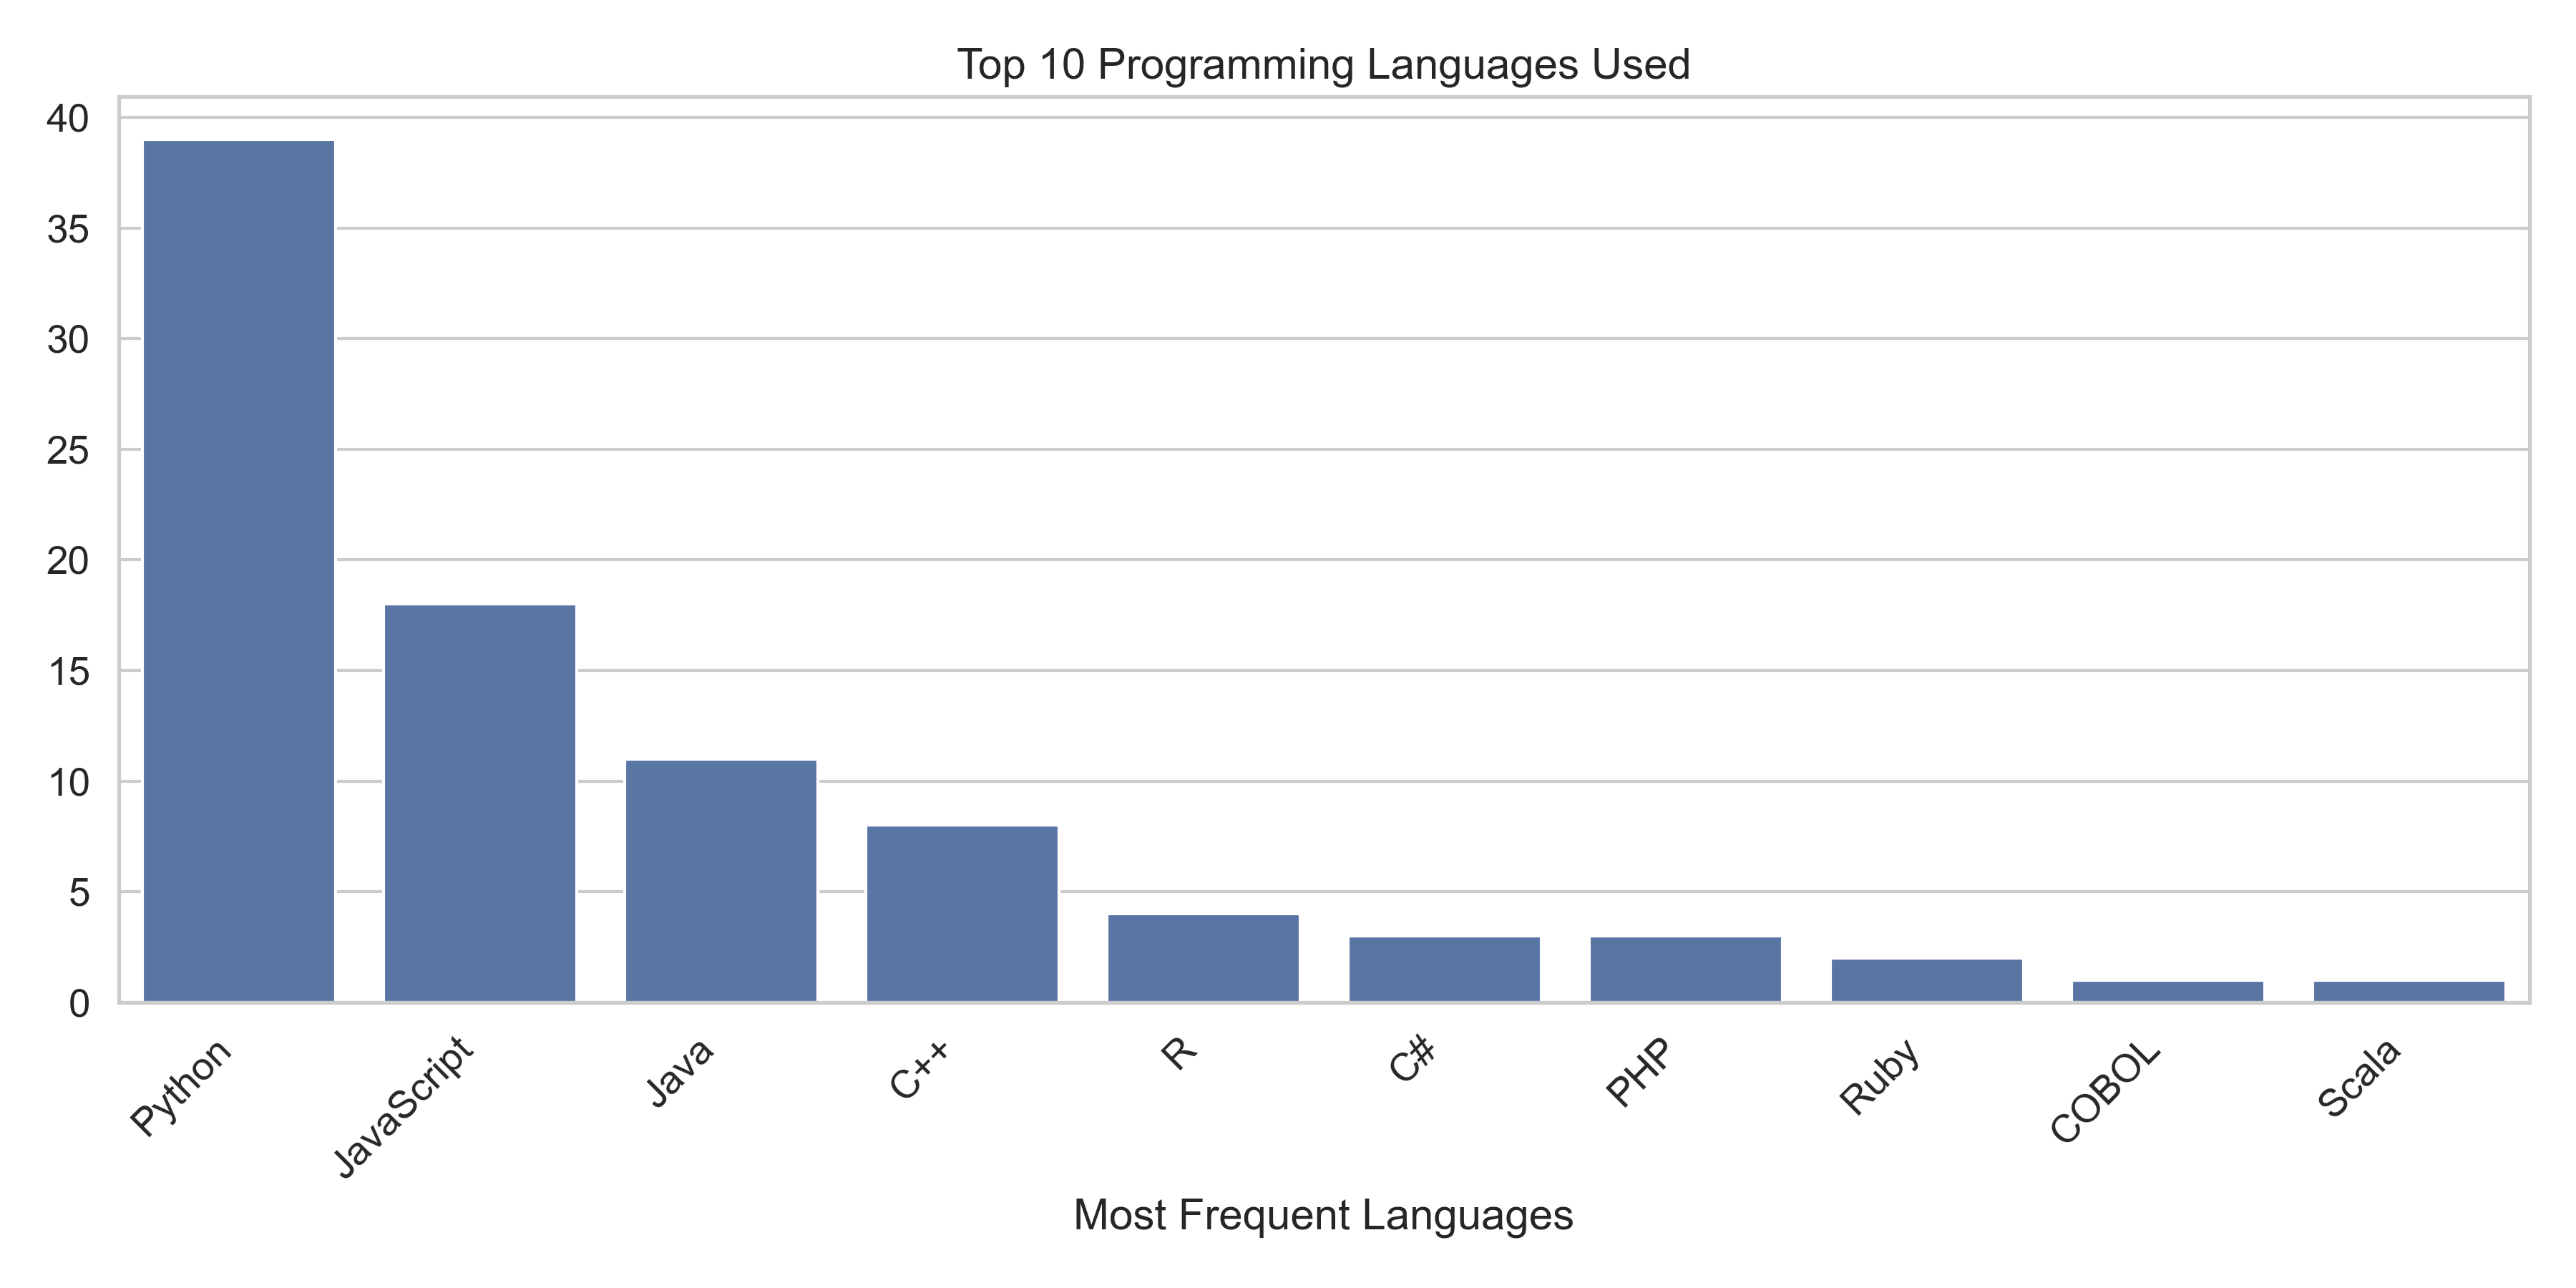
\includegraphics[width=0.8\linewidth]{final_research/language_distribution.png}
    \caption{Distribution of most frequently used programming languages}
    \label{fig:language_distribution}
\end{figure}

\subsection{AI Tool Adoption and Usage Patterns}
Our analysis revealed significant variations in AI tool adoption and usage frequencies across different demographics. ChatGPT emerged as the most widely used AI coding tool (56.7\%), followed by GitHub Copilot (36.1\%), Codeium (14.4\%), Tabnine (12.4\%), and Replit AI (8.2\%).

\begin{figure}[H]
    \centering
    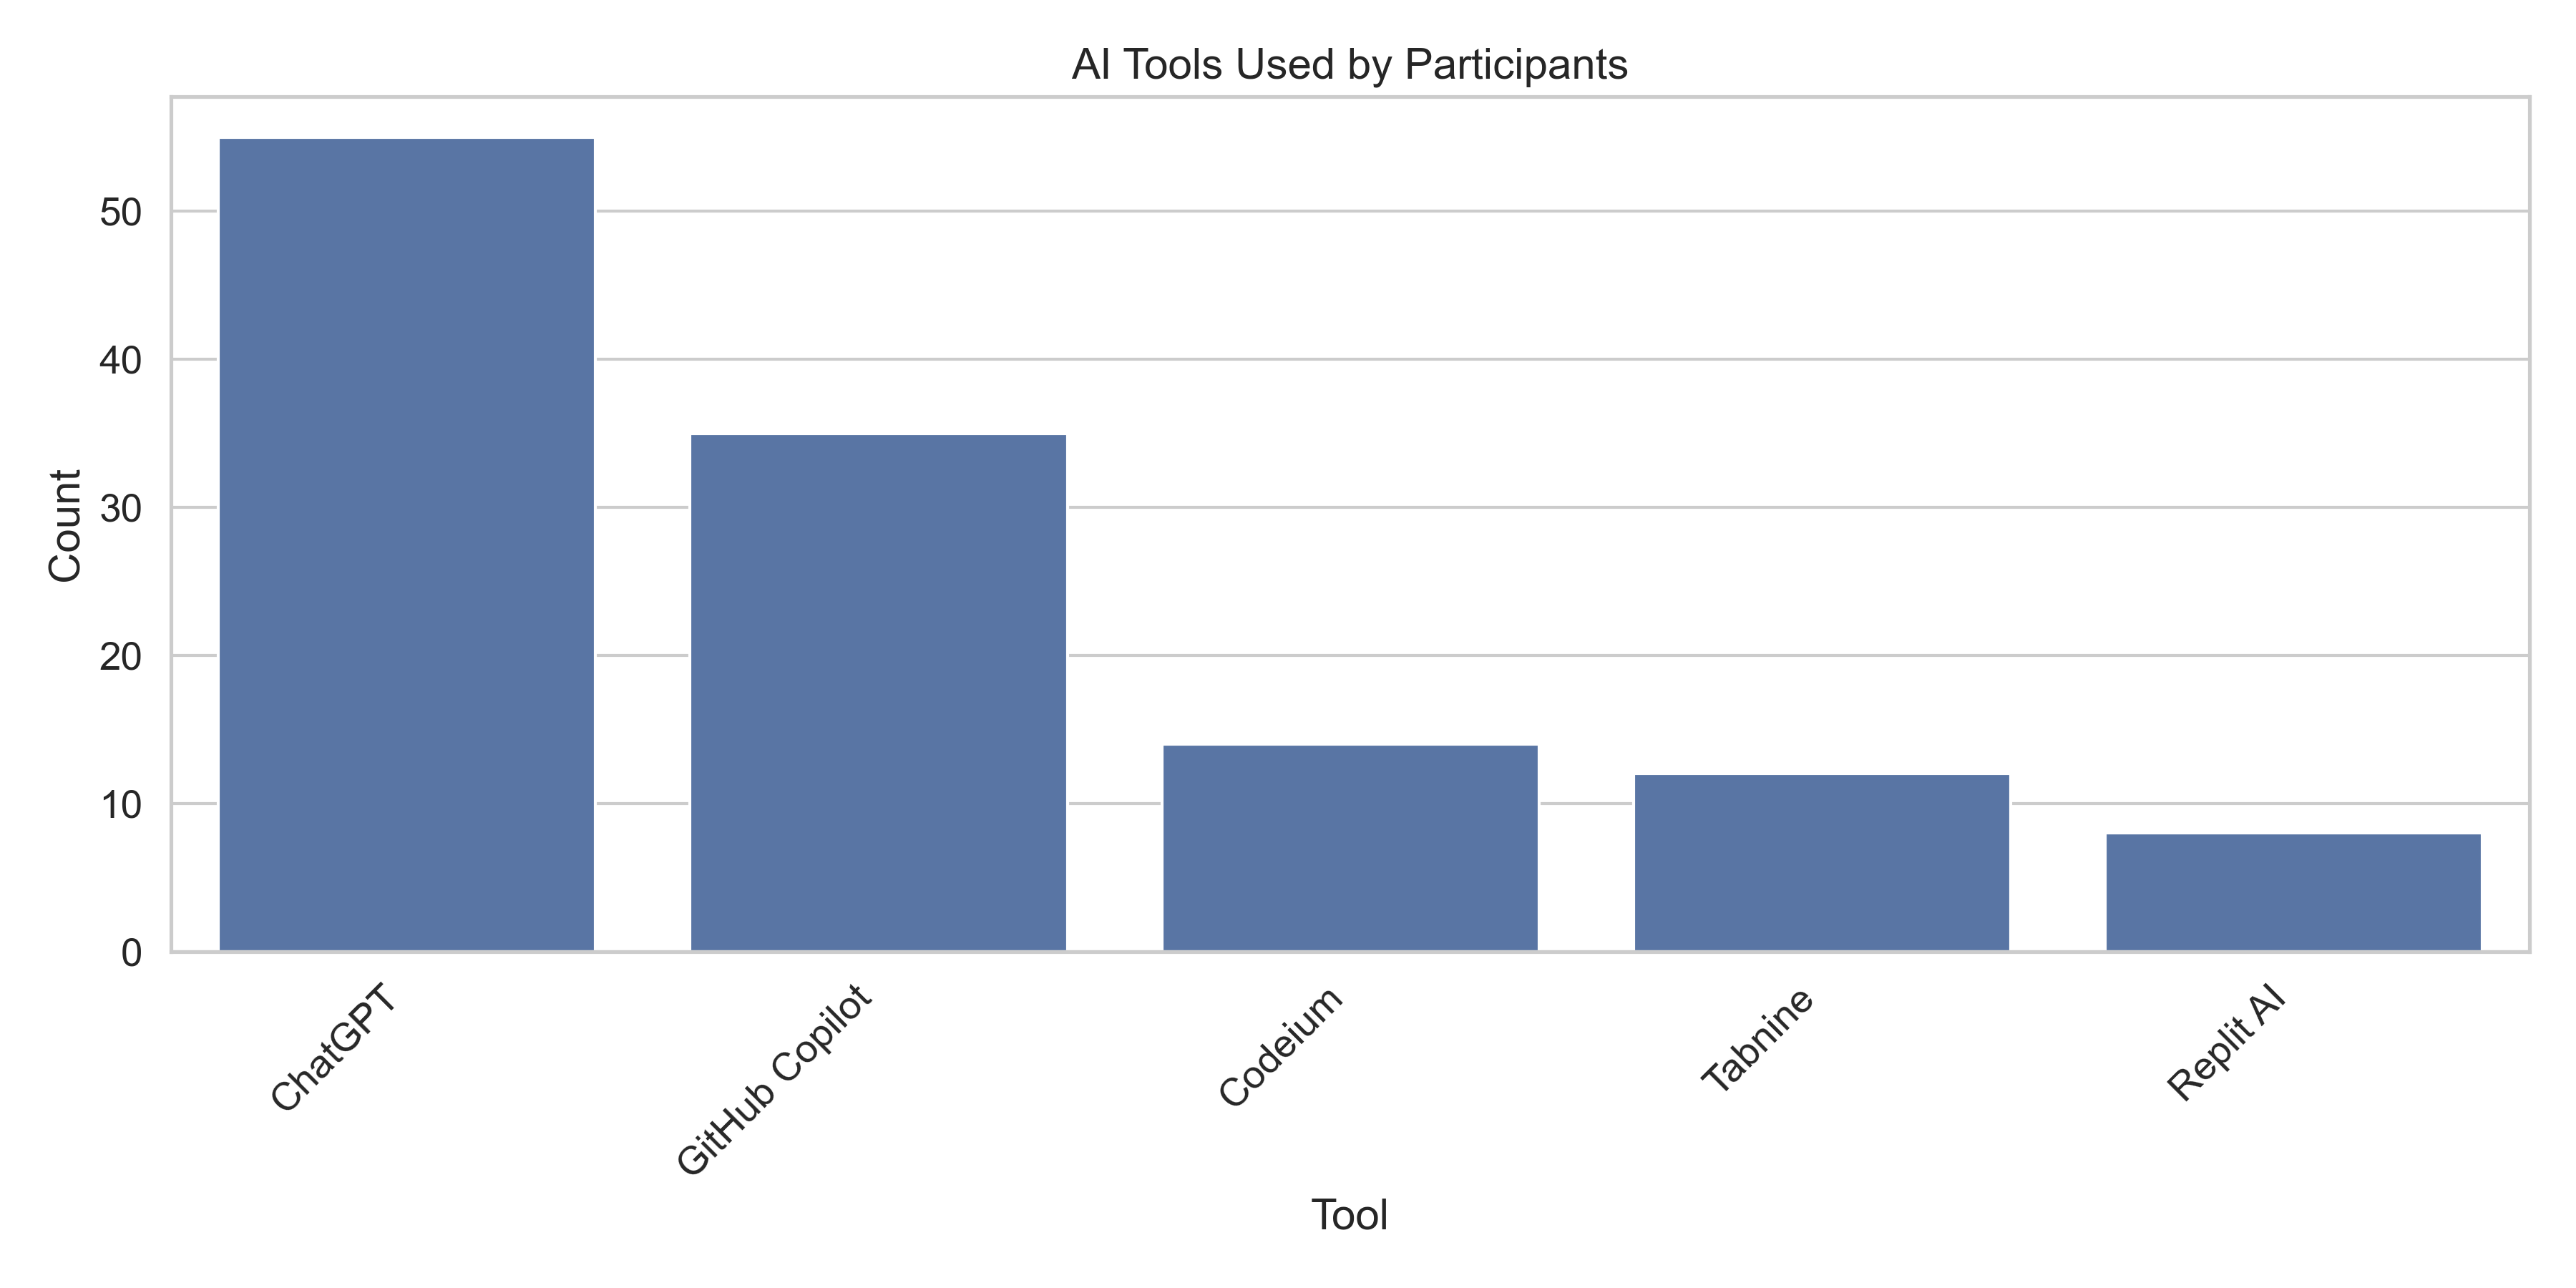
\includegraphics[width=0.8\linewidth]{final_research/tools_used.png}
    \caption{AI tools used by participants}
    \label{fig:tools_used}
\end{figure}

Usage frequency analysis showed that 41.2\% of participants use AI tools occasionally, 29.9\% use them weekly, and 28.9\% incorporate these tools into their daily workflow. Cross-tabulation analysis revealed distinct patterns across professional roles:
\begin{itemize}
    \item Data Scientists/ML Engineers had the highest daily usage rate (56.3\%)
    \item Freelancers primarily used AI tools weekly (63.6\%)
    \item Researchers had a more balanced distribution across daily, weekly, and occasional use
    \item Software Developers showed more occasional usage (50\%)
    \item Students overwhelmingly used AI tools occasionally (87\%), with only 13\% reporting weekly use
\end{itemize}

\begin{figure}[H]
    \centering
    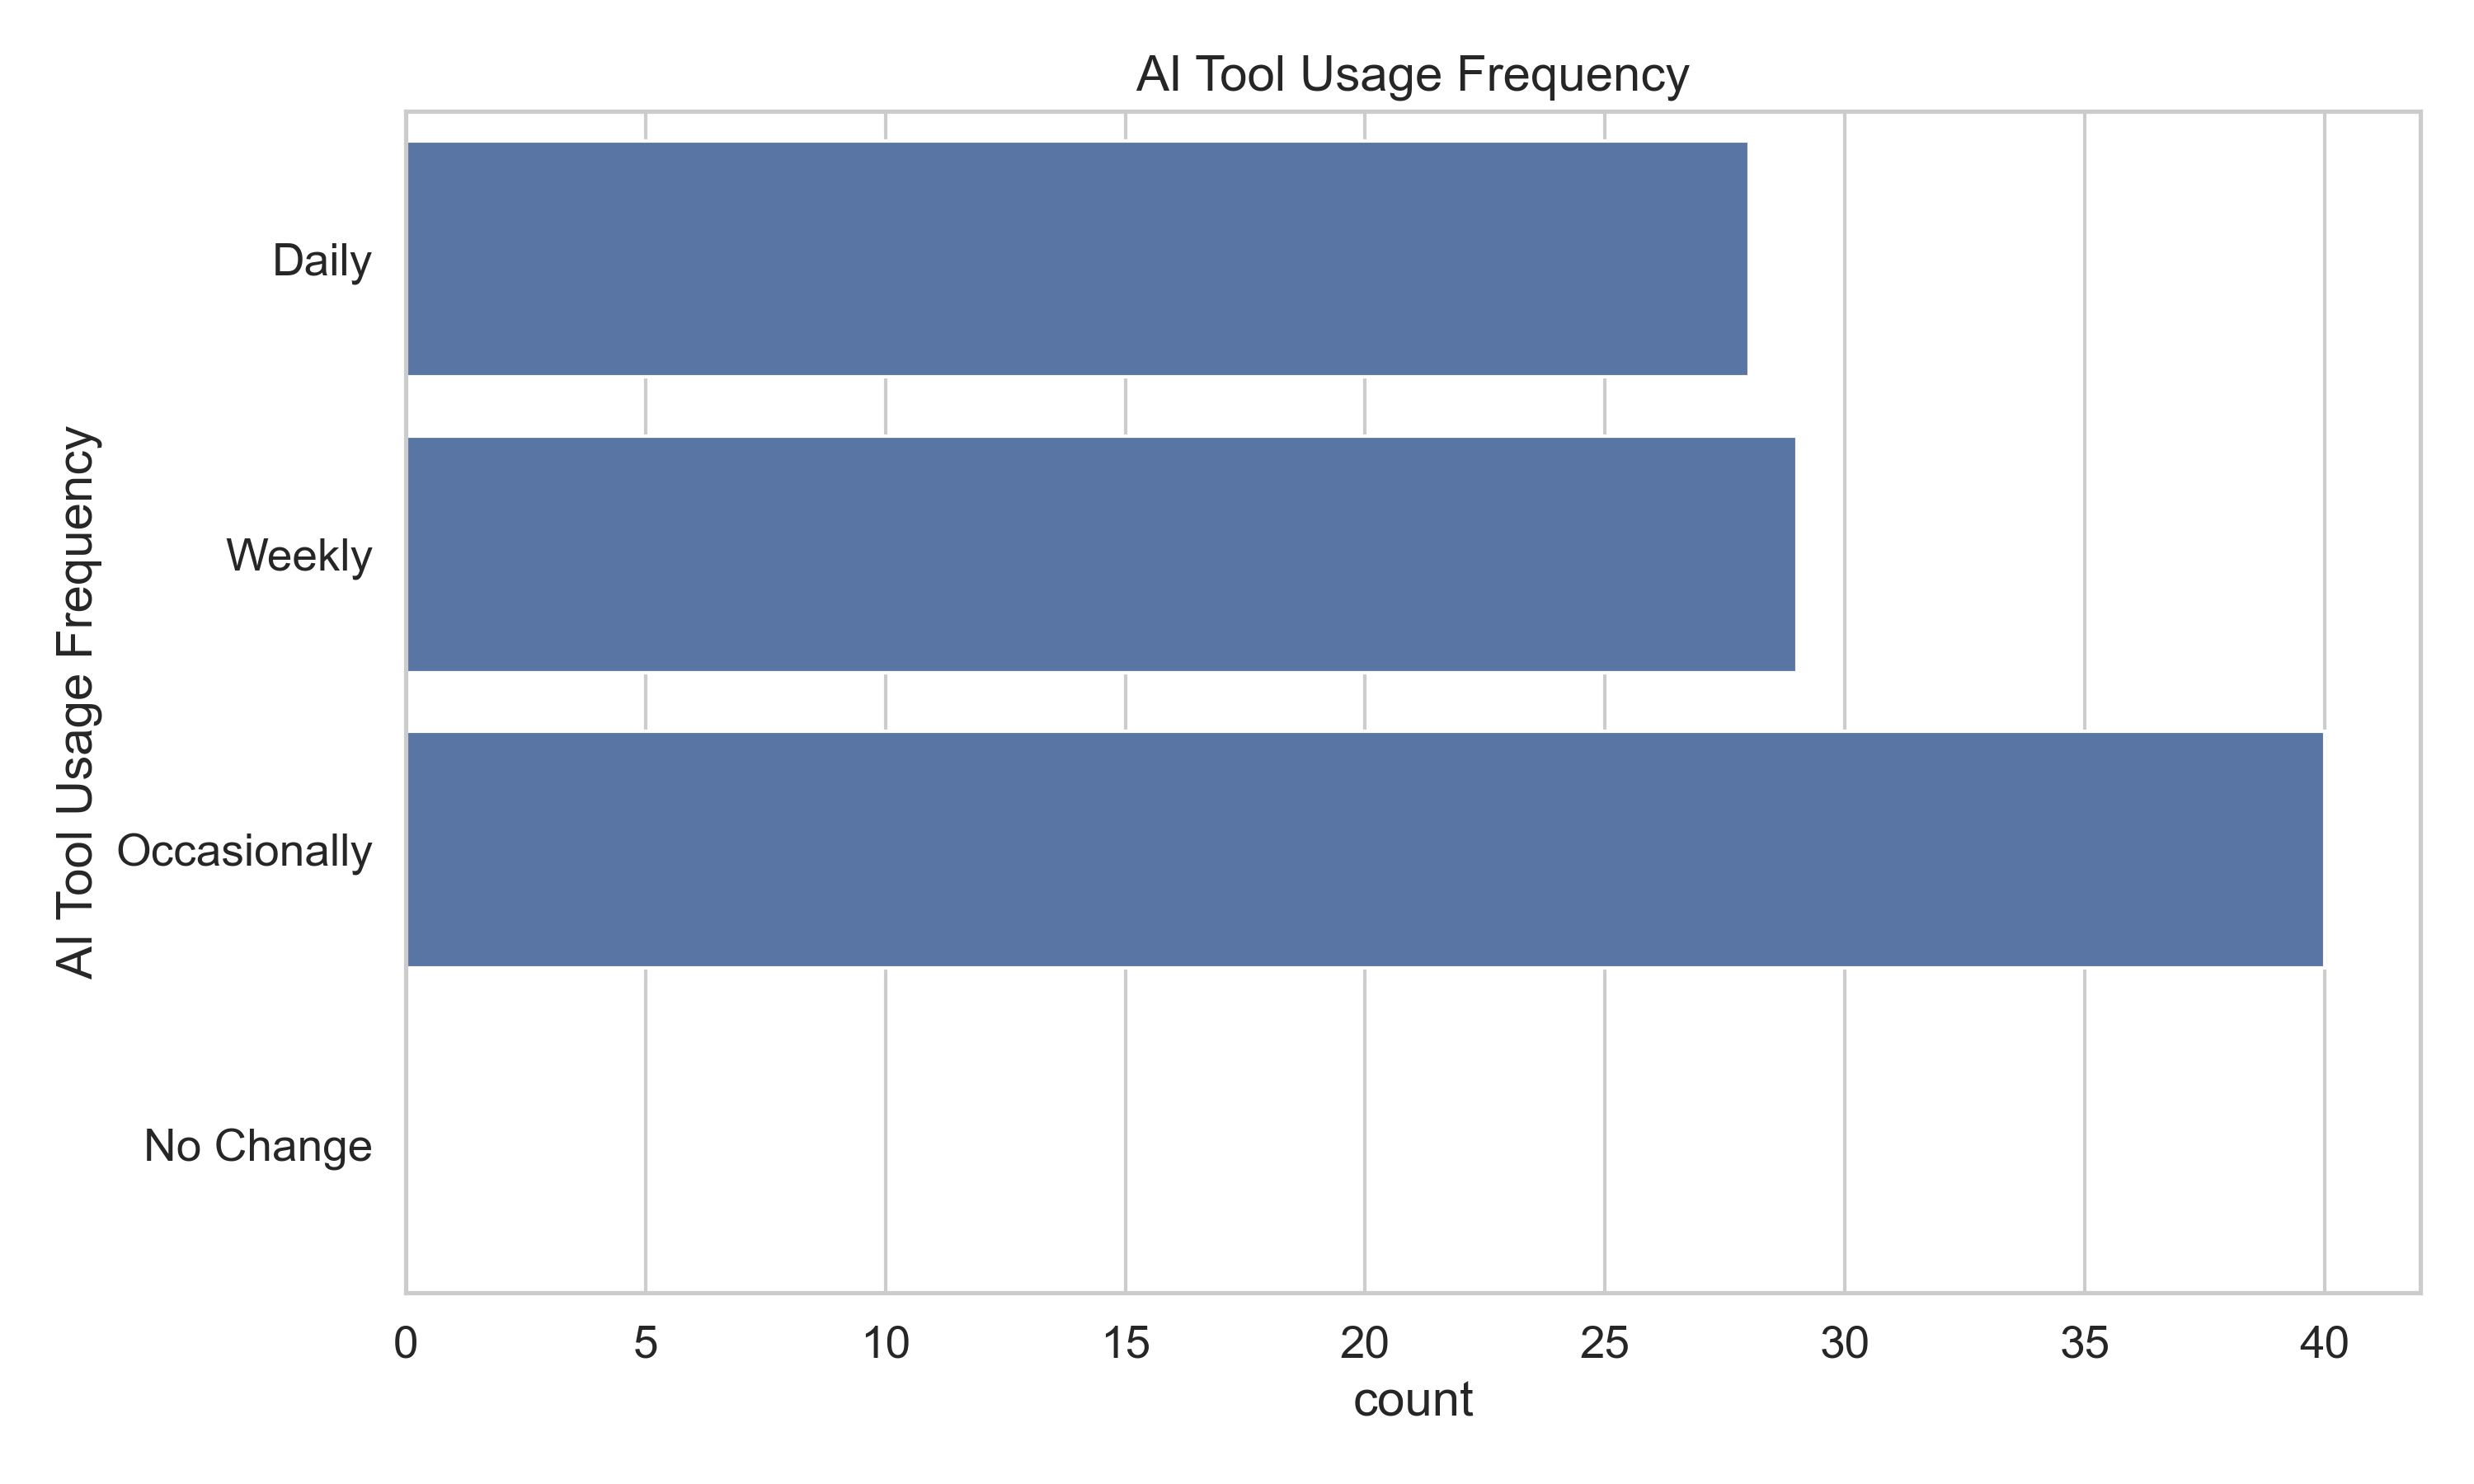
\includegraphics[width=0.8\linewidth]{final_research/usage_frequency.png}
    \caption{AI tool usage frequency}
    \label{fig:usage_frequency}
\end{figure}

The disparity in adoption rates highlights potential differences in workflow integration, tool accessibility, and perceived value across different professional contexts.

\subsection{Impact on Productivity and Code Quality}
AI coding tools demonstrated a significant positive impact on both productivity and code quality across many participant groups. Trust level in AI-generated code showed a strong correlation with reported productivity improvements:
\begin{itemize}
    \item Users reporting trust levels of 4-5 (on a 5-point scale) exclusively reported significant increases in coding speed
    \item Users with trust level 3 universally reported slight increases in coding speed
    \item Those with trust levels 1-2 reported no change in productivity
\end{itemize}

\begin{figure}[H]
    \centering
    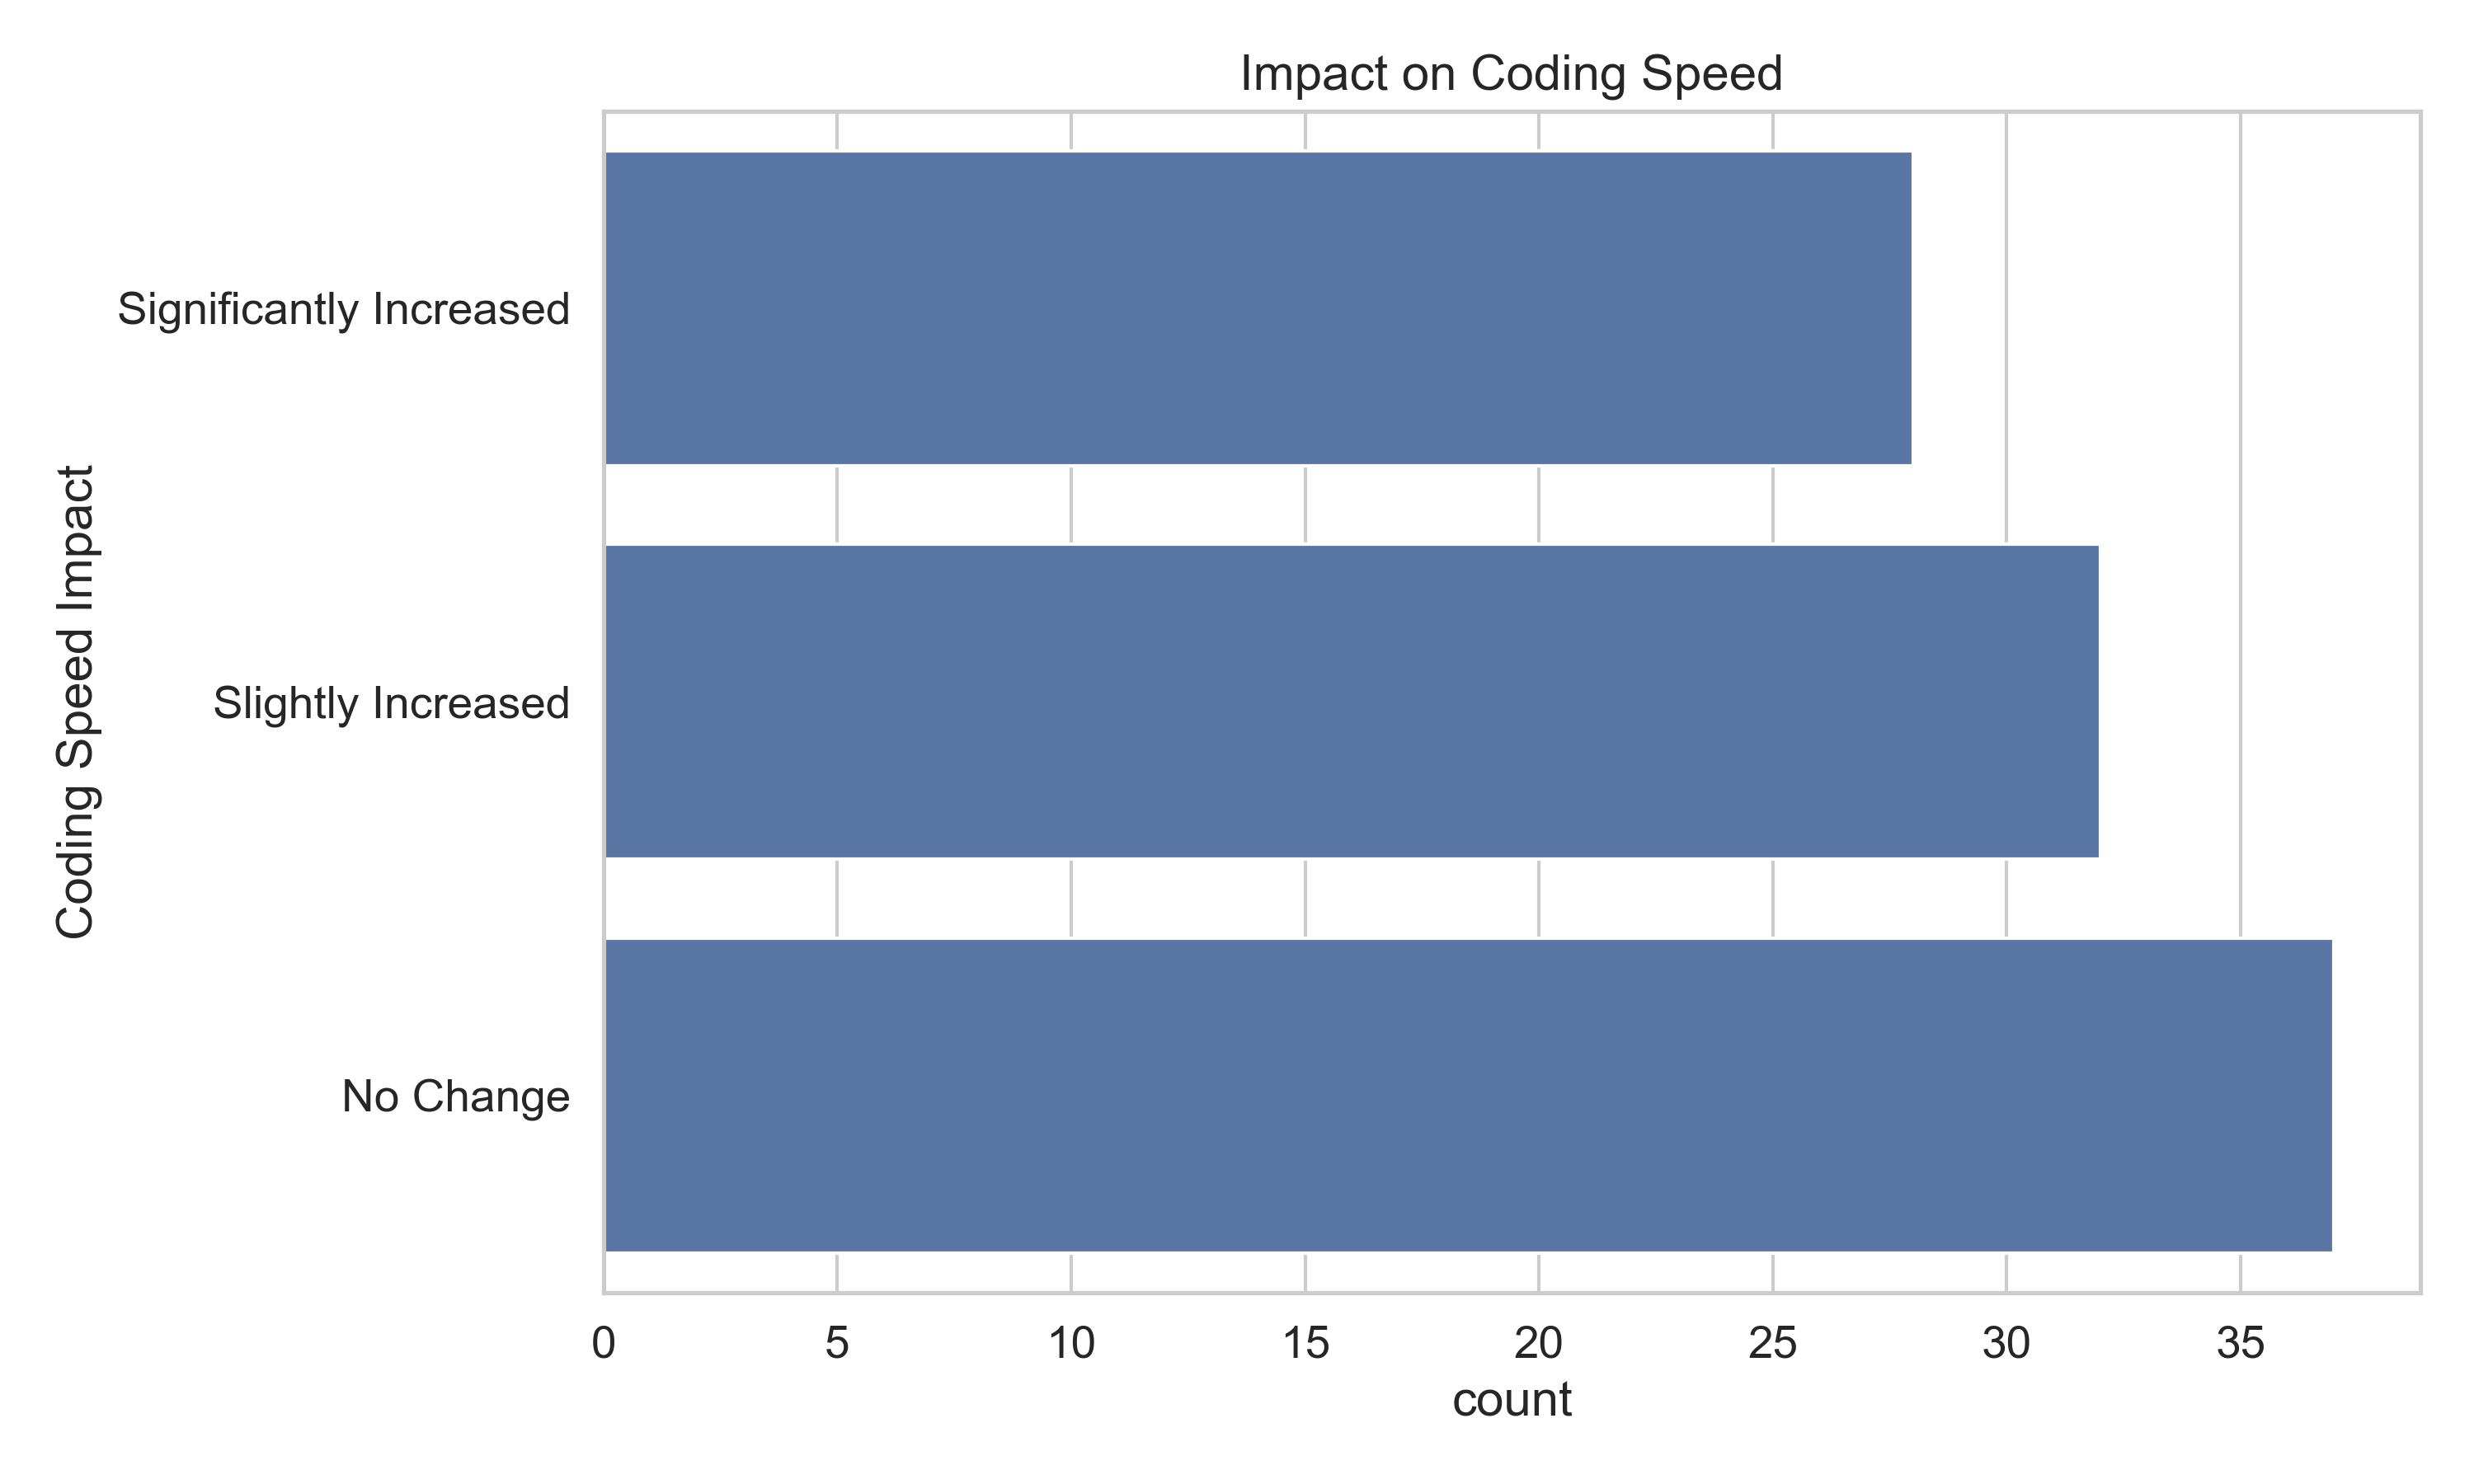
\includegraphics[width=0.8\linewidth]{final_research/coding_speed_impact.png}
    \caption{Impact of AI tools on coding speed}
    \label{fig:coding_speed_impact}
\end{figure}

\begin{figure}[H]
    \centering
    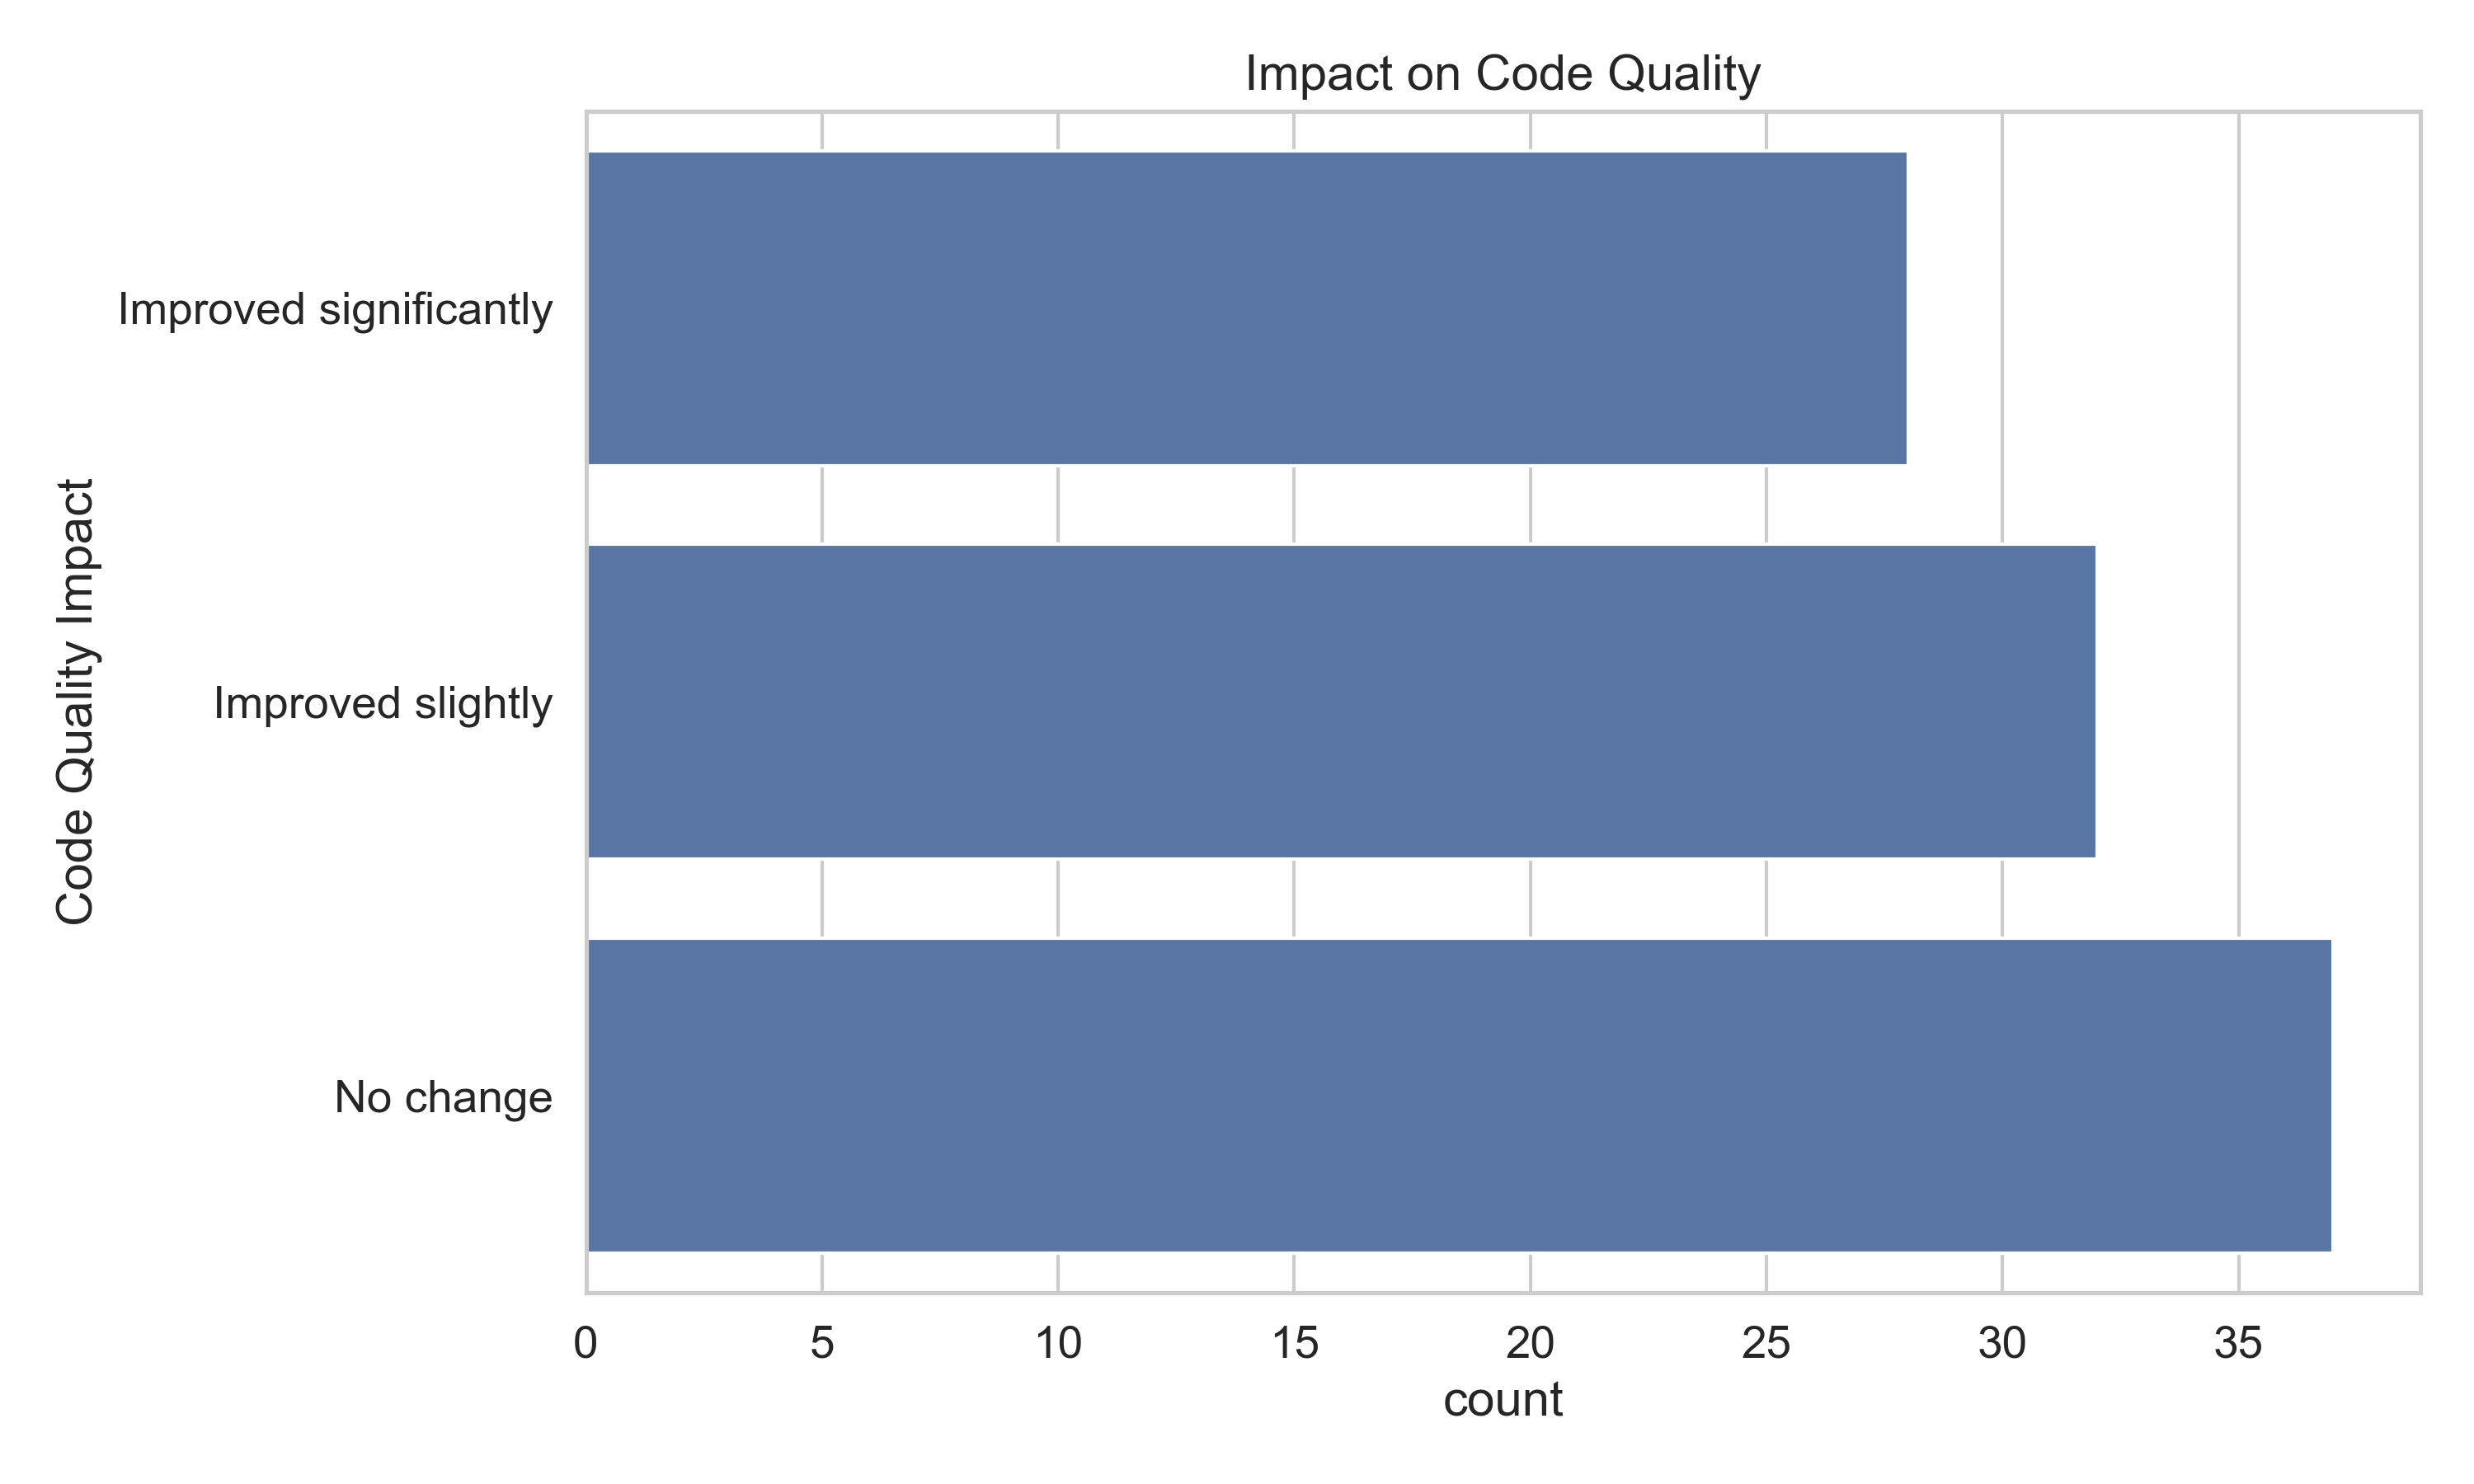
\includegraphics[width=0.8\linewidth]{final_research/code_quality_impact.png}
    \caption{Impact of AI tools on code quality}
    \label{fig:code_quality_impact}
\end{figure}

Examining the impact by professional role revealed that:
\begin{itemize}
    \item Software developers reported the highest rates of significant productivity increase (50\%)
    \item Freelancers predominantly experienced slightly increased productivity (63.6\%) 
    \item Students showed the least productivity impact, with 73.9\% reporting no change
    \item Data Scientists reported substantial productivity gains, with 56.3\% experiencing significant increases
\end{itemize}

Code quality improvements followed similar patterns, with higher trust levels correlating with perceived improvements in output quality. This suggests that comfort and confidence with AI tools might be a prerequisite for realizing their full productivity benefits.

\begin{table}[H]
    \caption{Relationship Between Trust Level and Coding Speed Impact}
    \centering
    \begin{tabular}{lccc}
        \toprule
        \textbf{Trust Level} & \textbf{No Change} & \textbf{Slightly Increased} & \textbf{Significantly Increased} \\
        \midrule
        1 & 100.0\% & 0.0\% & 0.0\% \\
        2 & 100.0\% & 0.0\% & 0.0\% \\
        3 & 0.0\% & 100.0\% & 0.0\% \\
        4 & 0.0\% & 0.0\% & 100.0\% \\
        5 & 0.0\% & 0.0\% & 100.0\% \\
        \bottomrule
    \end{tabular}
    \label{tab:trust_speed}
\end{table}

\subsection{Trust Levels and Concerns}
Trust in AI-generated code showed notable variations across different experience levels:
\begin{itemize}
    \item Among developers with 7+ years of experience, 51.1\% reported high trust (level 4), while 34.0\% reported low trust (level 1)
    \item Those with 4-6 years of experience overwhelmingly reported moderate trust (96.3\% at level 3)
    \item Less experienced professionals (1-3 years and less than 1 year) predominantly reported lower trust levels (76.9\% and 70\% at level 2 respectively)
\end{itemize}

\begin{figure}[H]
    \centering
    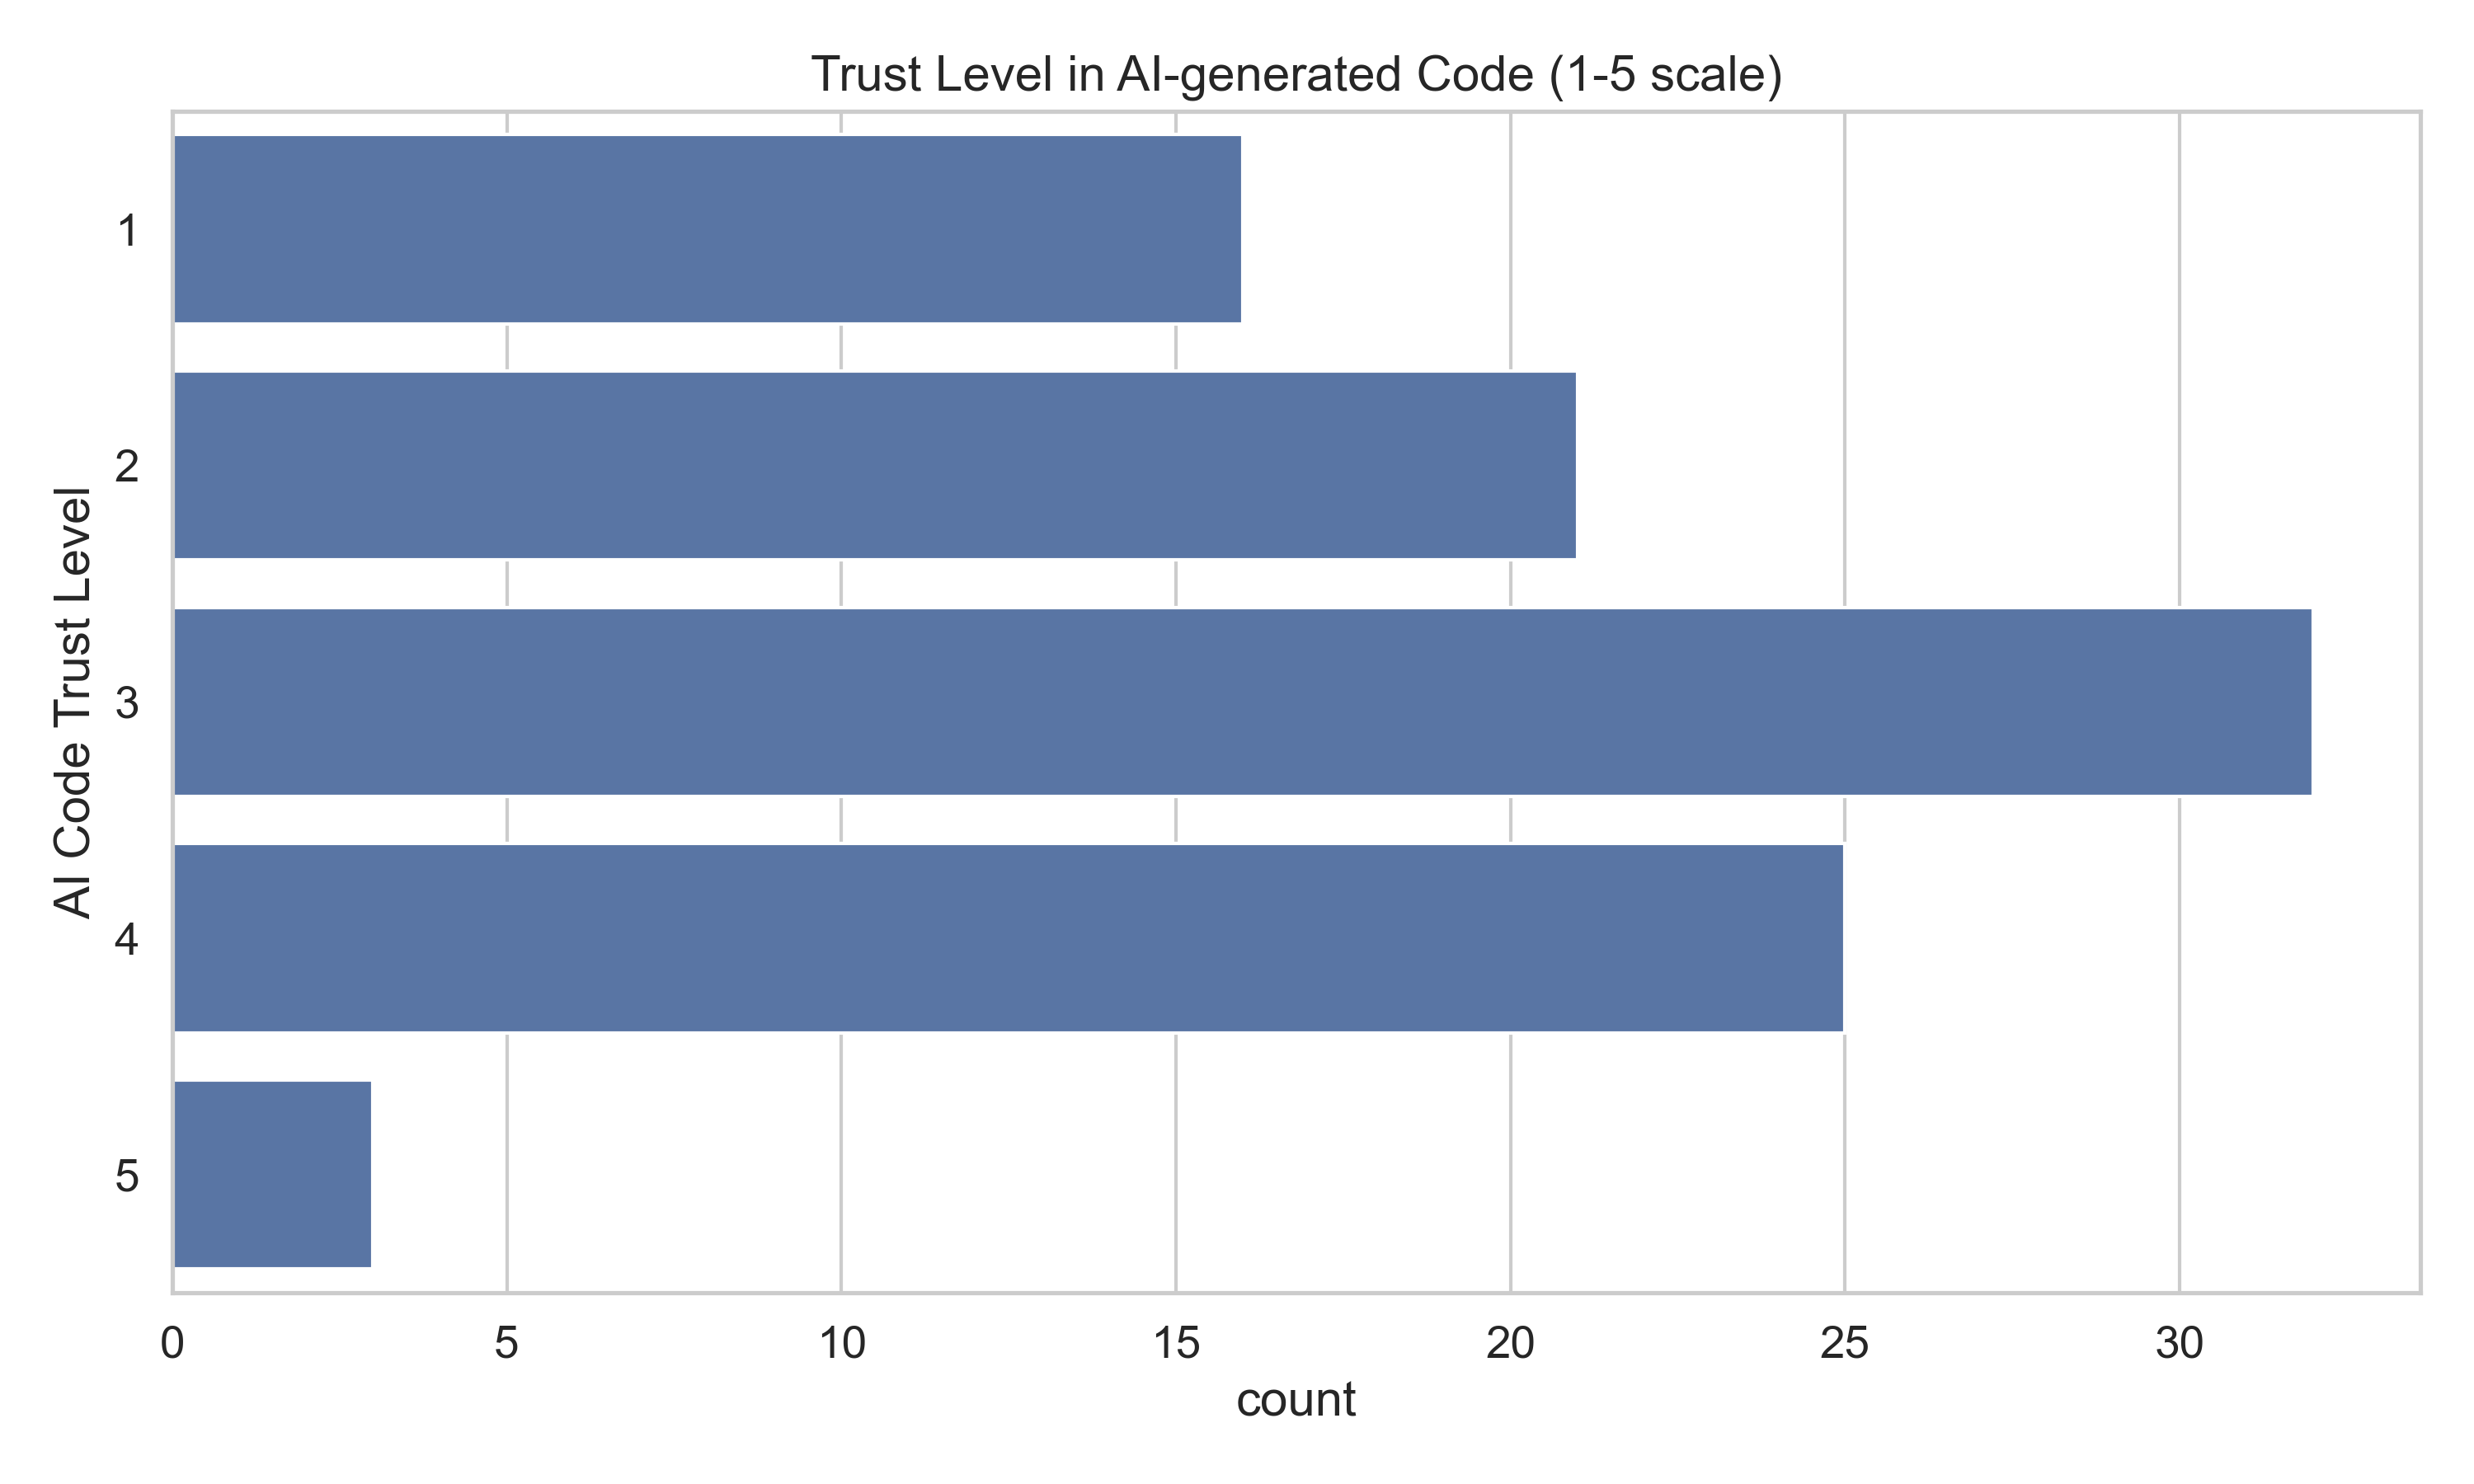
\includegraphics[width=0.8\linewidth]{final_research/trust_level.png}
    \caption{Trust levels in AI-generated code (1-5 scale)}
    \label{fig:trust_level}
\end{figure}

These variations suggest that experienced developers polarize into either high-trust adopters or skeptical users, while those with intermediate experience maintain a cautiously optimistic stance.

Concerns about AI coding tools varied significantly by professional role:
\begin{itemize}
    \item Software Developers expressed the most concern about AI replacing jobs (50\%) and dependency on AI (25\%)
    \item Students were primarily concerned about bias in AI-generated code (78.3\%)
    \item Researchers unanimously worried about plagiarism and copyright issues (100\%)
    \item Freelancers consistently expressed concerns about security risks (100\%)
    \item Data Scientists showed the least concerns overall, with 56.3\% reporting no concerns
\end{itemize}

\begin{figure}[H]
    \centering
    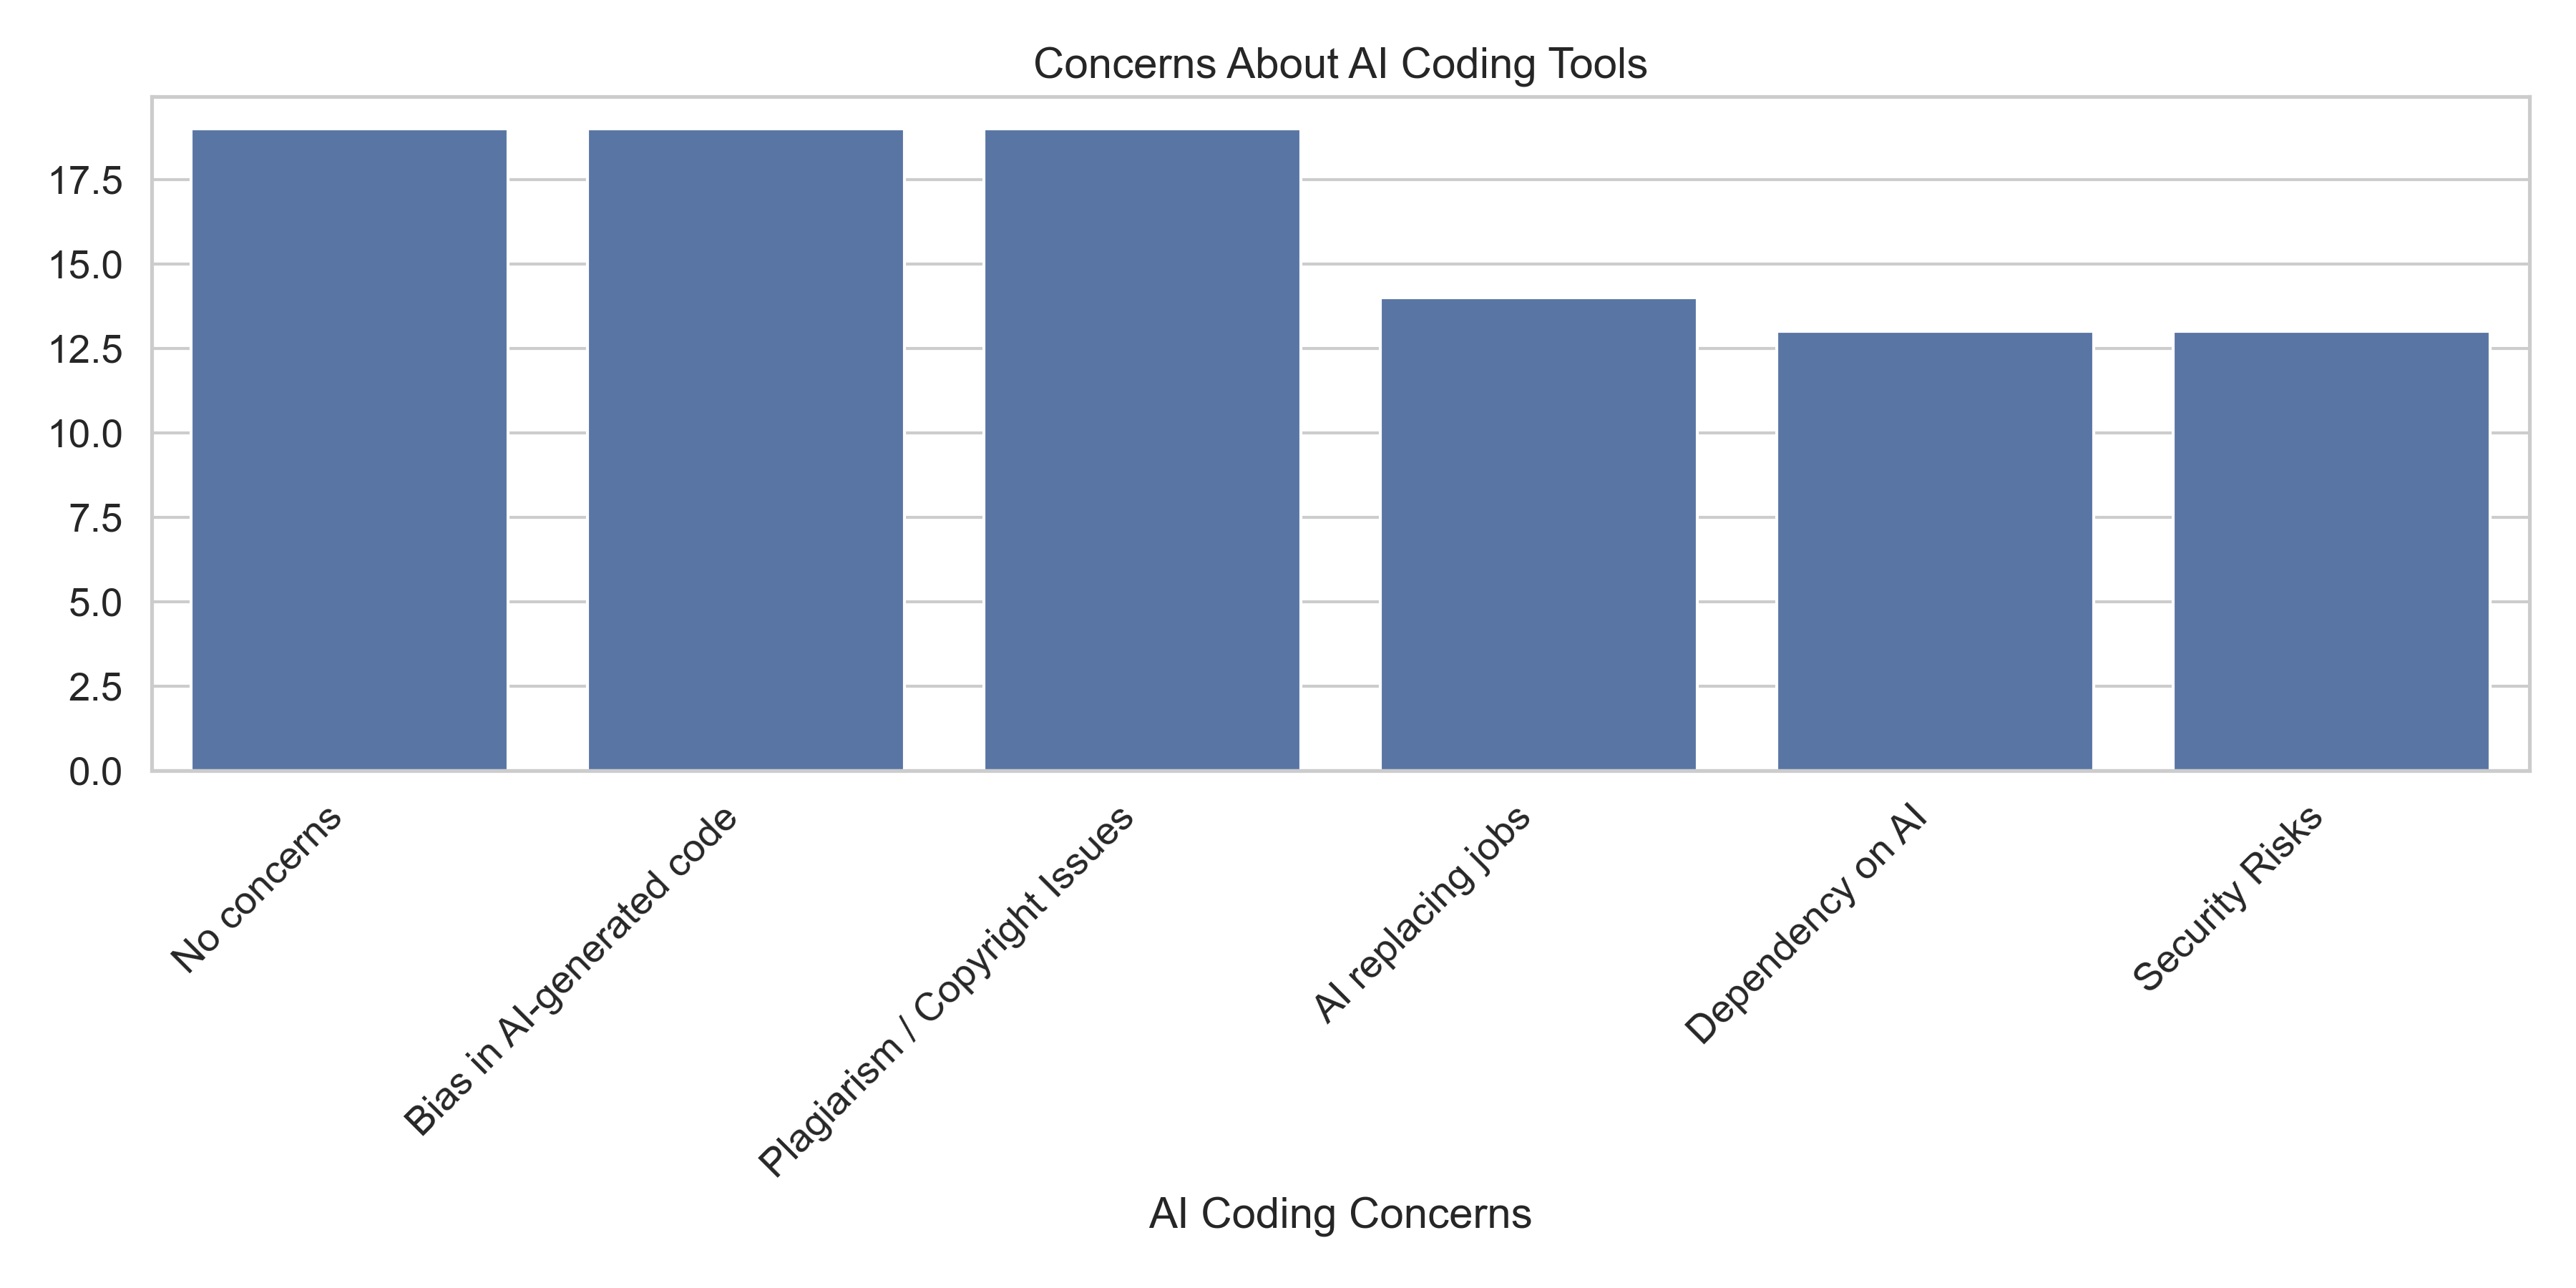
\includegraphics[width=0.8\linewidth]{final_research/concerns.png}
    \caption{Concerns about AI coding tools}
    \label{fig:concerns}
\end{figure}

The distribution of concerns reflects the specific challenges and priorities of each professional context, from academic integrity for researchers to security for client-facing freelance work.

\begin{table}[H]
    \caption{AI Coding Concerns by Professional Role (Percentage)}
    \centering
    \resizebox{\textwidth}{!}{%
    \begin{tabular}{lcccccc}
        \toprule
        \textbf{Role} & \textbf{Replacing Jobs} & \textbf{Bias} & \textbf{Dependency} & \textbf{No Concerns} & \textbf{Plagiarism} & \textbf{Security} \\
        \midrule
        Data Scientist & 0.0 & 6.3 & 37.5 & 56.3 & 0.0 & 0.0 \\
        Freelancer & 0.0 & 0.0 & 0.0 & 0.0 & 0.0 & 100.0 \\
        Researcher & 0.0 & 0.0 & 0.0 & 0.0 & 100.0 & 0.0 \\
        Software Developer & 50.0 & 0.0 & 25.0 & 17.9 & 0.0 & 7.1 \\
        Student & 0.0 & 78.3 & 0.0 & 21.7 & 0.0 & 0.0 \\
        \bottomrule
    \end{tabular}%
    }
    \label{tab:role_concerns}
\end{table}

\subsection{Creativity and Innovation Impact}
Perceptions regarding AI's impact on creativity showed intriguing patterns, with most participants recognizing positive effects. The survey identified three primary views on creativity impact:
\begin{enumerate}
    \item Enhanced creativity by automating repetitive tasks
    \item Encouraged innovation by suggesting new approaches
    \item Reduced creativity by making developers overly reliant on AI
\end{enumerate}

\begin{figure}[H]
    \centering
    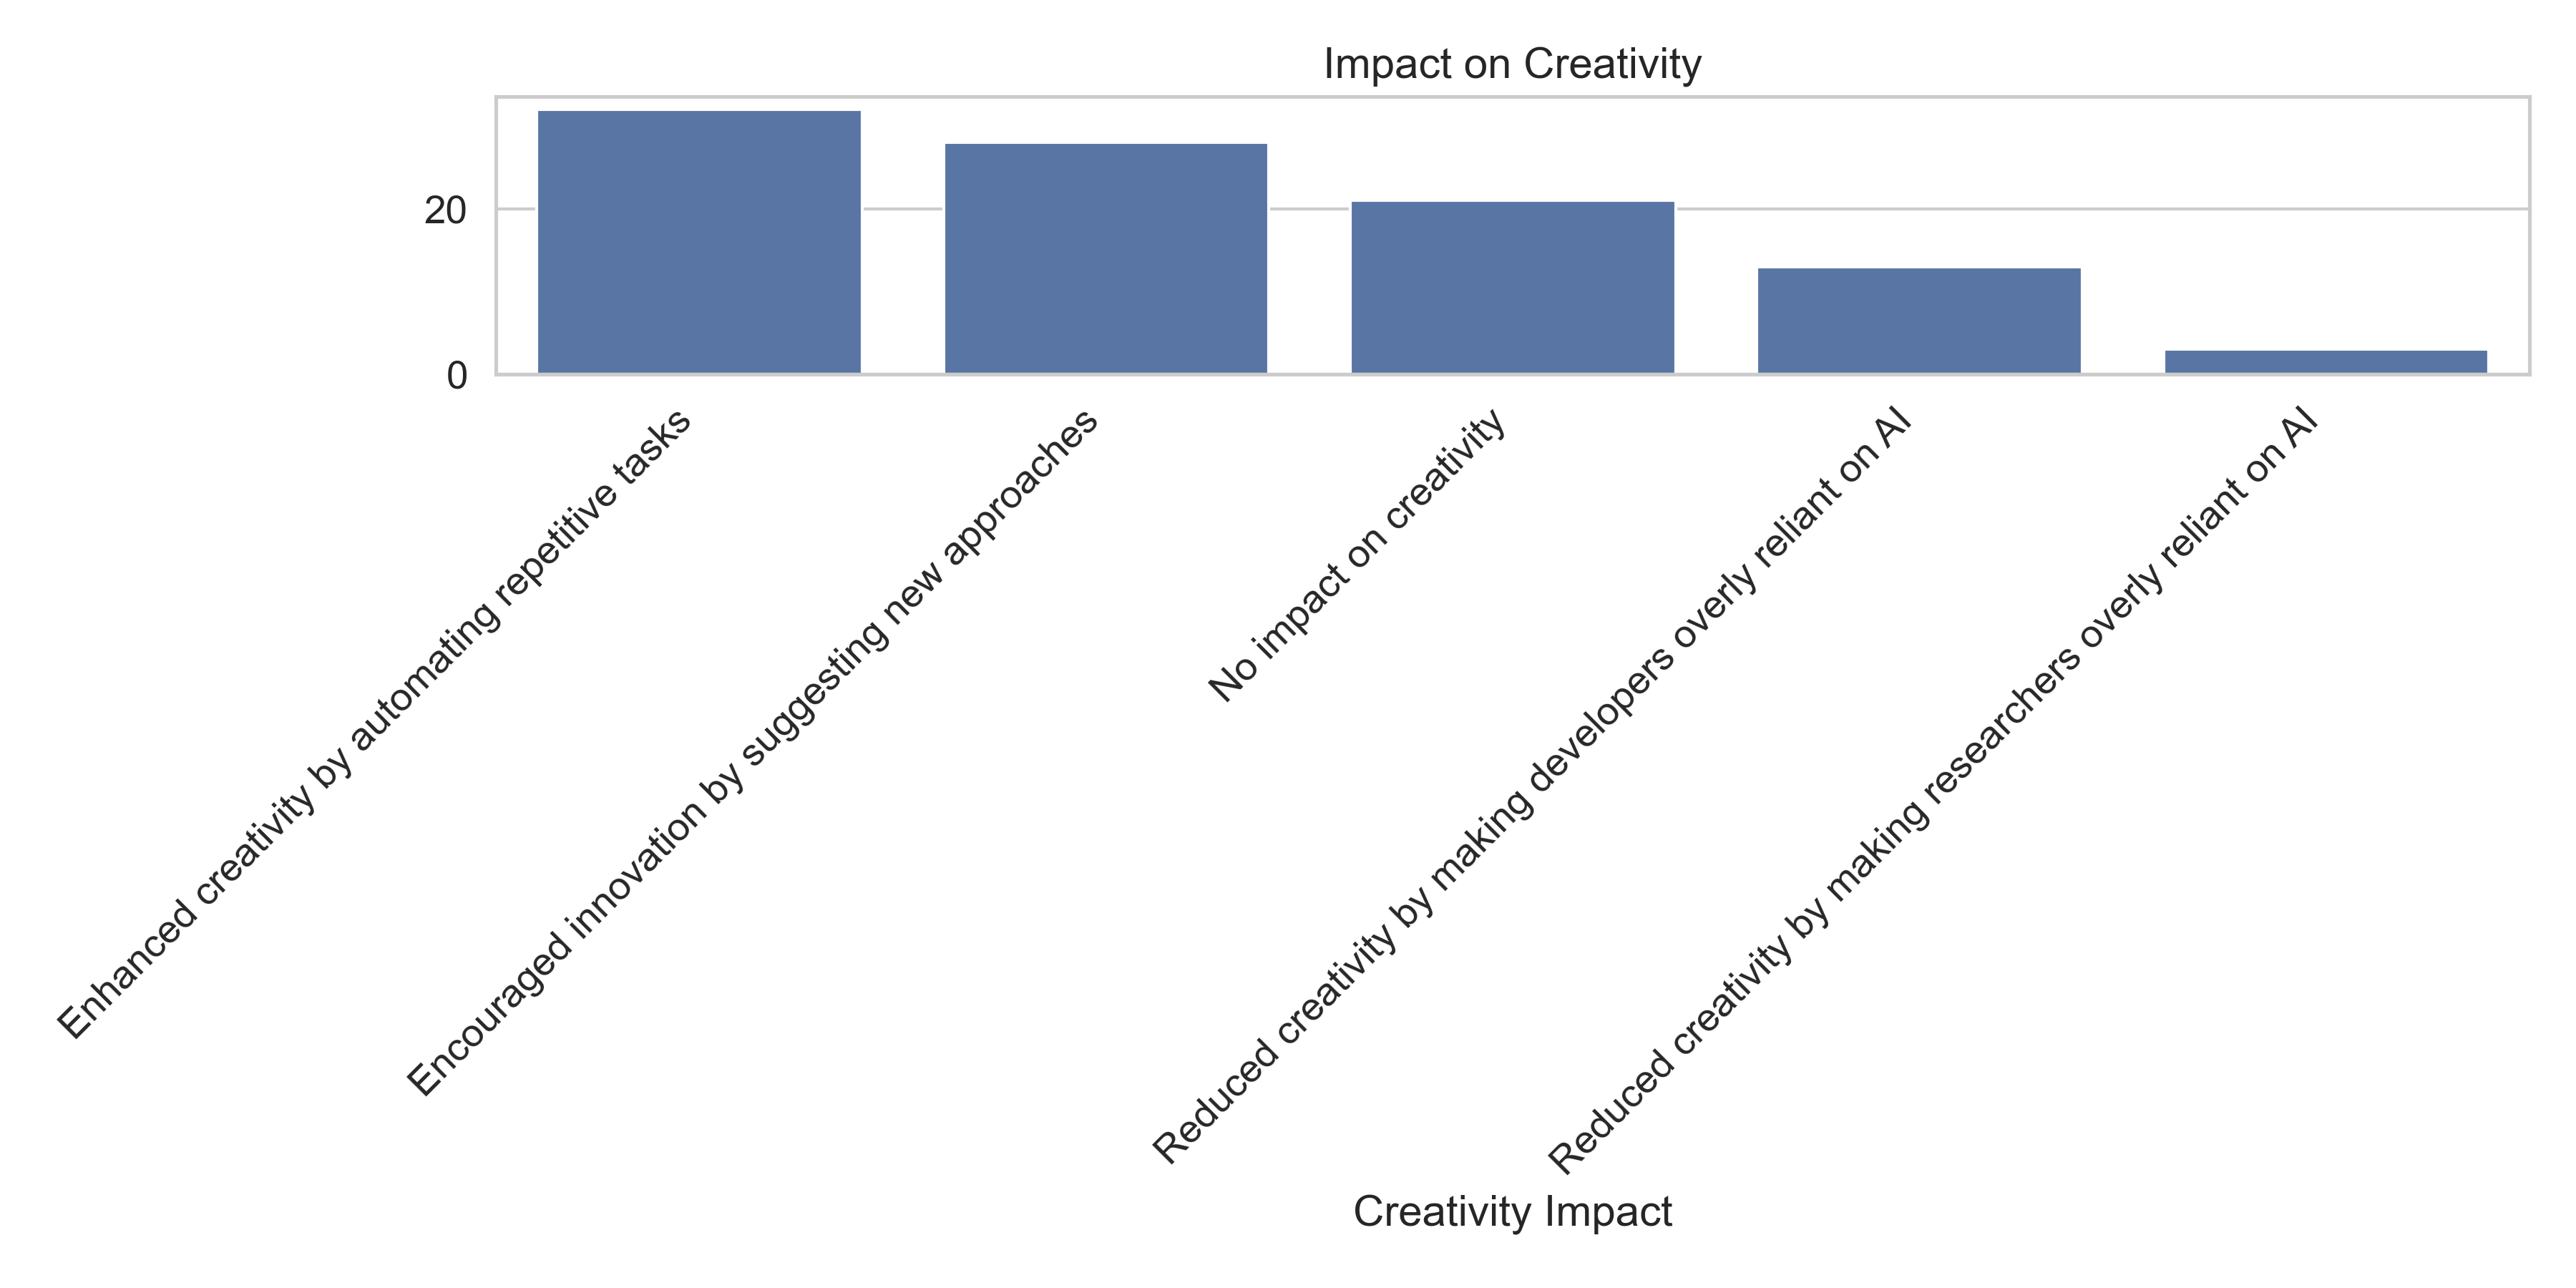
\includegraphics[width=0.8\linewidth]{final_research/creativity_impact.png}
    \caption{Perceived impact of AI tools on creativity}
    \label{fig:creativity_impact}
\end{figure}

The distribution of these perceptions correlated strongly with trust levels and usage frequency, with daily users more likely to report innovation enhancement and occasional users more likely to express concerns about reduced creativity.

Experience level also played a role in creativity perception:
\begin{itemize}
    \item More experienced developers (7+ years) were divided between perceiving enhanced innovation (among those with high trust) and reduced creativity (among those with low trust)
    \item Mid-career professionals (4-6 years) consistently reported that AI enhanced creativity by automating routine tasks
    \item Less experienced coders showed mixed perceptions, with some reporting enhanced creativity and others reporting no impact
\end{itemize}

\subsection{Future Software Capabilities}
Analysis of participants' requests for autonomous software capabilities revealed six major categories of desired tools:
\begin{enumerate}
    \item Learning tools (25.8\%): Personalized learning platforms, adaptive assessment systems, and interactive visualization tools
    \item Research tools (20.6\%): Paper analysis engines, collaboration platforms, and citation management systems
    \item Development tools (19.6\%): Project management, architecture design, and workflow optimization systems
    \item Data analysis tools (12.4\%): Predictive analytics, visualization platforms, and data processing pipelines
    \item Specialized systems (8.2\%): Healthcare diagnostics, legacy system modernization, and vertical-specific applications
    \item Security-focused tools (3.1\%): Secure document management and security-enhanced project platforms
\end{enumerate}

\begin{figure}[H]
    \centering
    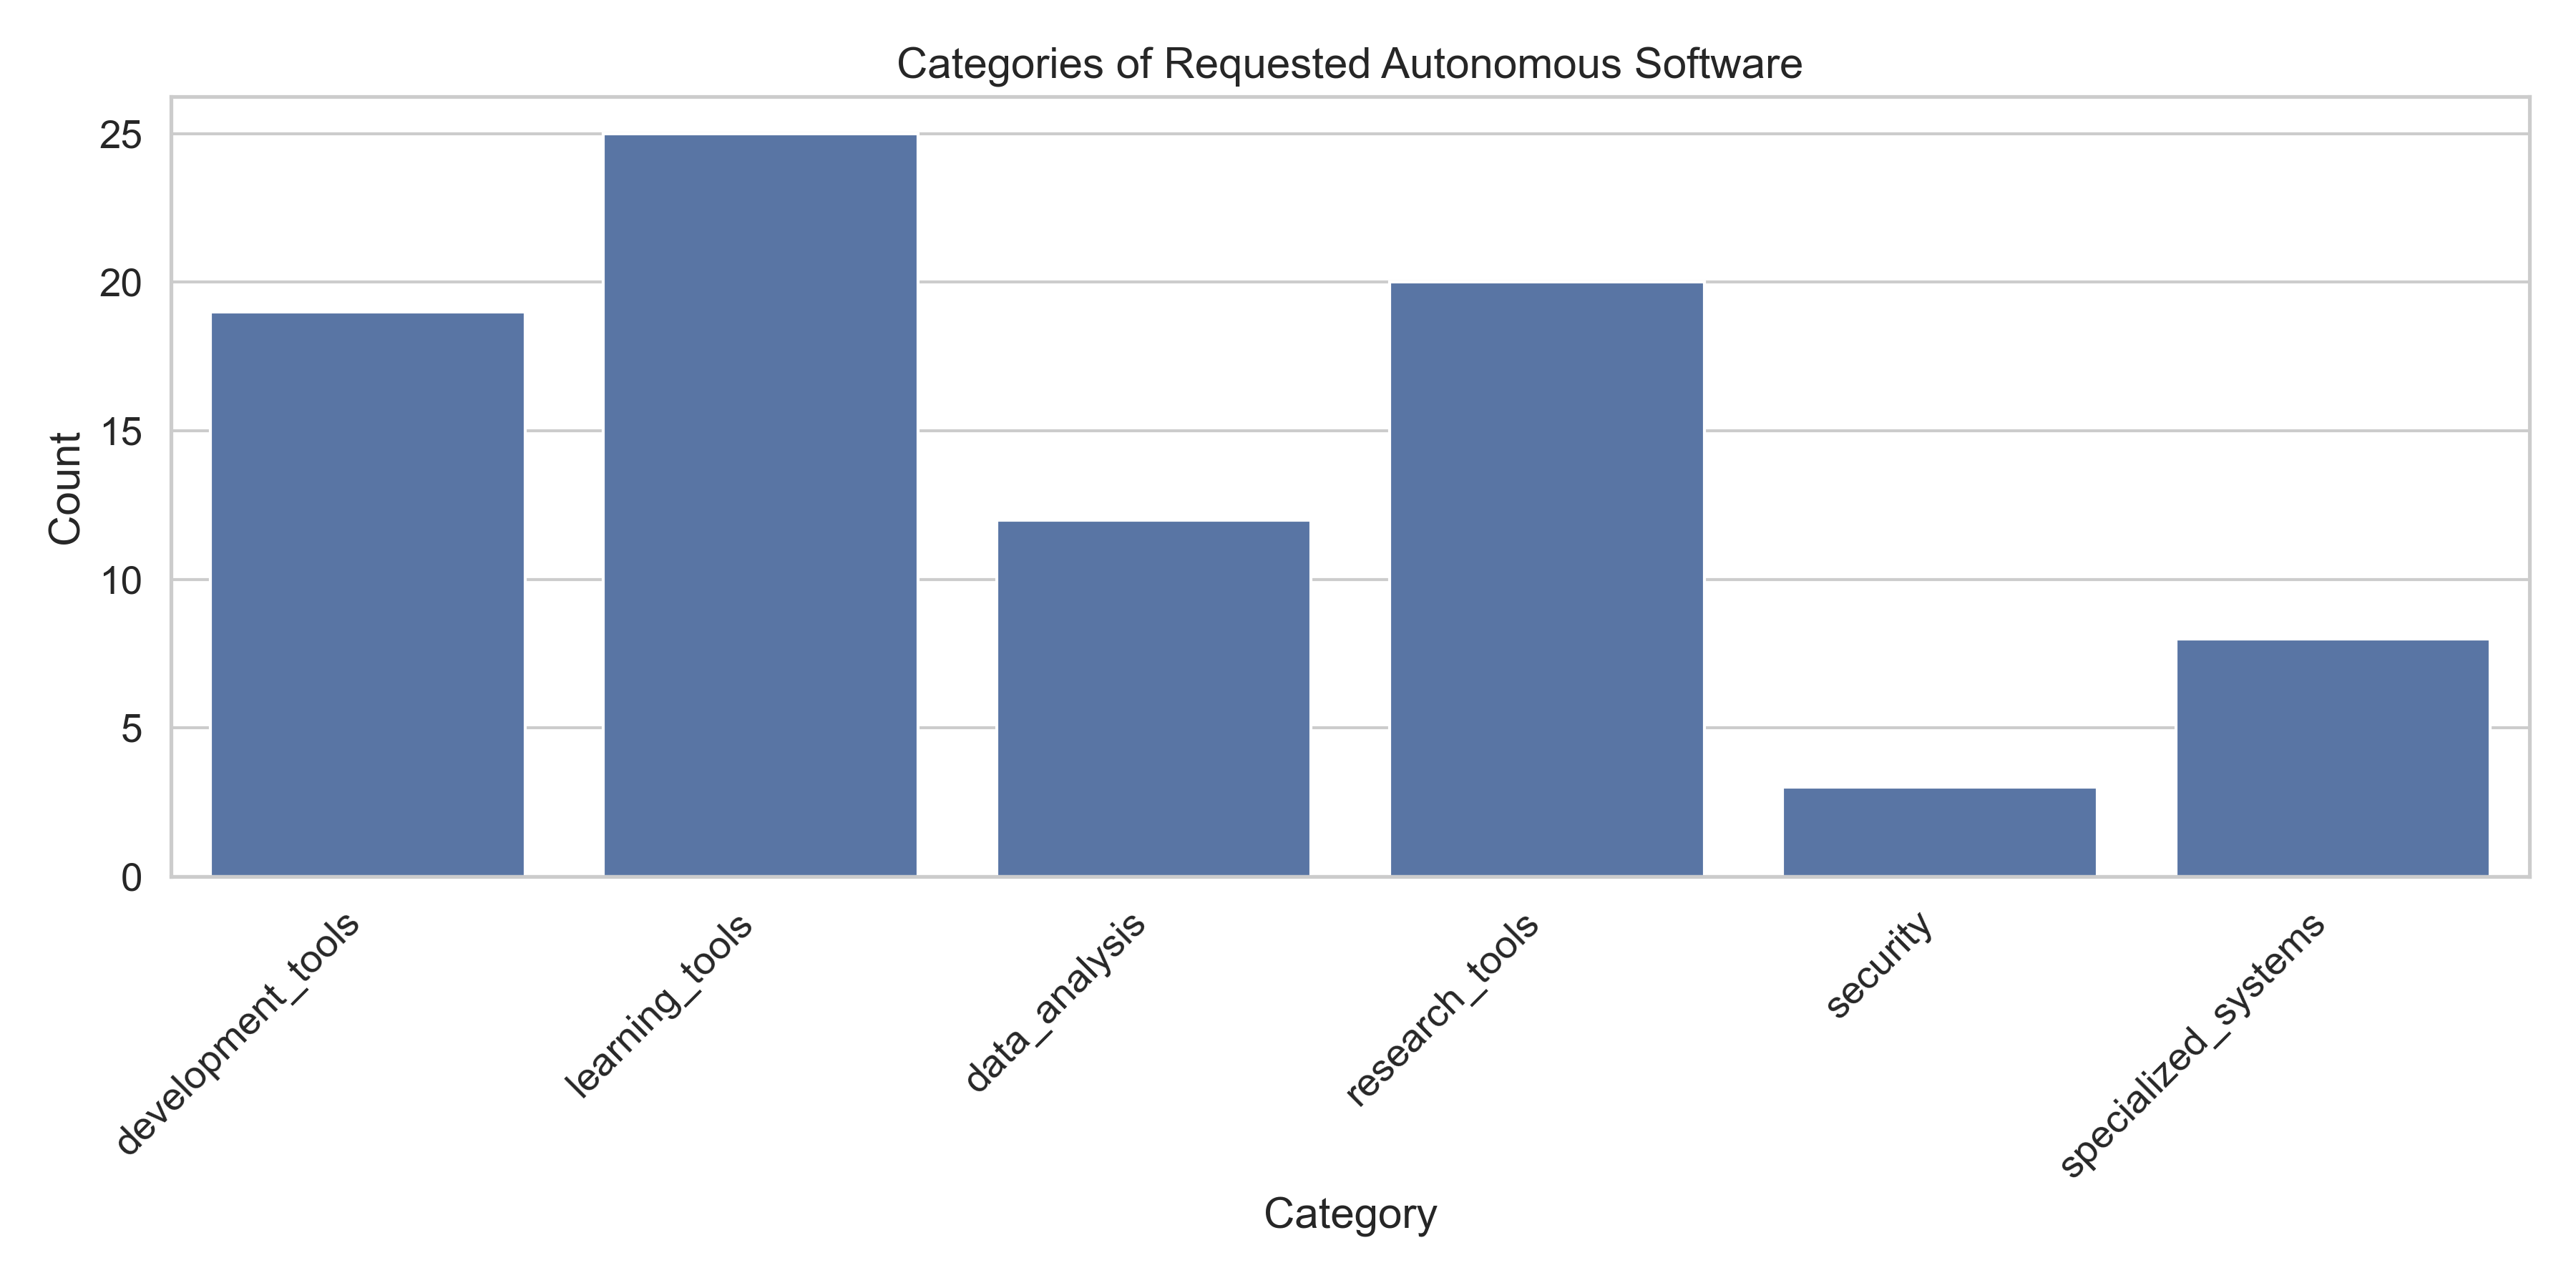
\includegraphics[width=0.8\linewidth]{final_research/software_request_categories.png}
    \caption{Categories of requested autonomous software}
    \label{fig:software_requests}
\end{figure}

The requested capabilities varied by professional role, with students prioritizing learning tools, researchers focusing on academic assistance, and developers seeking productivity enhancement and automation of routine tasks.

\section{Discussion}
\subsection{Key Insights}
Our analysis reveals several key insights into the adoption and impact of AI coding tools:

First, trust in AI-generated code appears to be a prerequisite for realizing productivity benefits, with a direct correlation between trust level and reported productivity improvements. This suggests that building user confidence may be as important as technical capability in driving effective AI tool adoption.

Second, experience level creates a polarizing effect on AI perception. The most experienced developers (7+ years) showed a bimodal distribution of trust levels, suggesting a division between enthusiastic adopters and skeptical traditionalists. This contrasts with mid-career professionals (4-6 years) who demonstrated more consistent moderate trust and positive perceptions.

Third, professional roles significantly influence both usage patterns and concerns. Data Scientists emerged as the most receptive to AI tools with high adoption rates and minimal concerns, likely due to their familiarity with AI technologies. Researchers, while active users, expressed unanimous concerns about plagiarism and attribution. Students, despite being digital natives, showed more cautious adoption patterns and significant concerns about bias.

Fourth, the relationship between AI tools and creativity is nuanced, with most users reporting that AI either enhances creativity through automation or encourages innovation through novel suggestions. This contradicts concerns that AI might diminish creative problem-solving abilities.

\subsection{Demographic Variations}
The data revealed significant demographic variations in AI tool perception and usage. Age groups showed distinct patterns:
\begin{itemize}
    \item Younger professionals (18-24) demonstrated cautious adoption with occasional usage
    \item Mid-career professionals (25-44) represented the most active and enthusiastic user segment
    \item Senior professionals (45+) showed more polarized views, either fully embracing or significantly questioning AI tools
\end{itemize}

Educational background also influenced adoption, with advanced degree holders (Ph.D. and Master's) more likely to incorporate AI tools into daily workflows compared to those with Bachelor's degrees or high school education.

These variations suggest that demographic factors play a substantial role in shaping attitudes toward and adoption of AI coding tools.

\subsection{Professional Role Differences}
Professional roles emerged as one of the strongest predictors of AI tool usage patterns and perceptions:

Data Scientists and ML Engineers exhibited the highest rates of daily use (56.3\%), significantly higher than the overall average (28.9\%). Their technical background and familiarity with AI technologies likely contributed to their comfort with these tools, resulting in higher trust levels and minimal concerns.

Freelancers showed a strong preference for weekly usage (63.6\%) and unanimously expressed security concerns, reflecting their client-focused work context and the importance of data protection in their professional relationships.

Researchers demonstrated balanced usage patterns but expressed unanimous concerns about plagiarism and copyright issues, highlighting the importance of academic integrity in their work.

Software Developers showed the highest productivity gains but also the most concern about job replacement (50\%), reflecting the direct relevance of AI coding tools to their core professional activities.

Students predominantly used AI tools occasionally (87\%) for learning purposes, with significant concerns about bias in AI-generated code (78.3\%), suggesting a more exploratory and educational approach to these technologies.

\subsection{Experience Level Influence}
Experience level demonstrated a compelling influence on AI tool perception:

The relationship between experience and trust in AI-generated code revealed an intriguing pattern. Less experienced coders (under 3 years) predominantly reported lower trust levels (70-77\% at level 2), while the most experienced developers (7+ years) showed a polarized distribution with 51.1\% reporting high trust (level 4) but 34.0\% reporting very low trust (level 1). Mid-career professionals (4-6 years) overwhelmingly reported moderate trust (96.3\% at level 3).

\begin{table}[H]
    \caption{Trust in AI-Generated Code by Experience Level (Percentage)}
    \centering
    \begin{tabular}{lccccc}
        \toprule
        \textbf{Experience} & \textbf{Trust 1} & \textbf{Trust 2} & \textbf{Trust 3} & \textbf{Trust 4} & \textbf{Trust 5} \\
        \midrule
        Less than 1 year & 0.0 & 70.0 & 30.0 & 0.0 & 0.0 \\
        1-3 years & 0.0 & 76.9 & 23.1 & 0.0 & 0.0 \\
        4-6 years & 0.0 & 0.0 & 96.3 & 3.7 & 0.0 \\
        7+ years & 34.0 & 8.5 & 0.0 & 51.1 & 6.4 \\
        \bottomrule
    \end{tabular}
    \label{tab:experience_trust}
\end{table}

Experience also strongly correlated with perceptions of AI potentially replacing human developers:
\begin{itemize}
    \item Among professionals with 7+ years of experience, 61.7\% believed human oversight would always be necessary
    \item Those with 4-6 years believed AI could replace humans but only for repetitive tasks (77.8\%)
    \item Less experienced coders unanimously expressed uncertainty about AI's future role (100\% selecting "Not sure")
\end{itemize}

\begin{figure}[H]
    \centering
    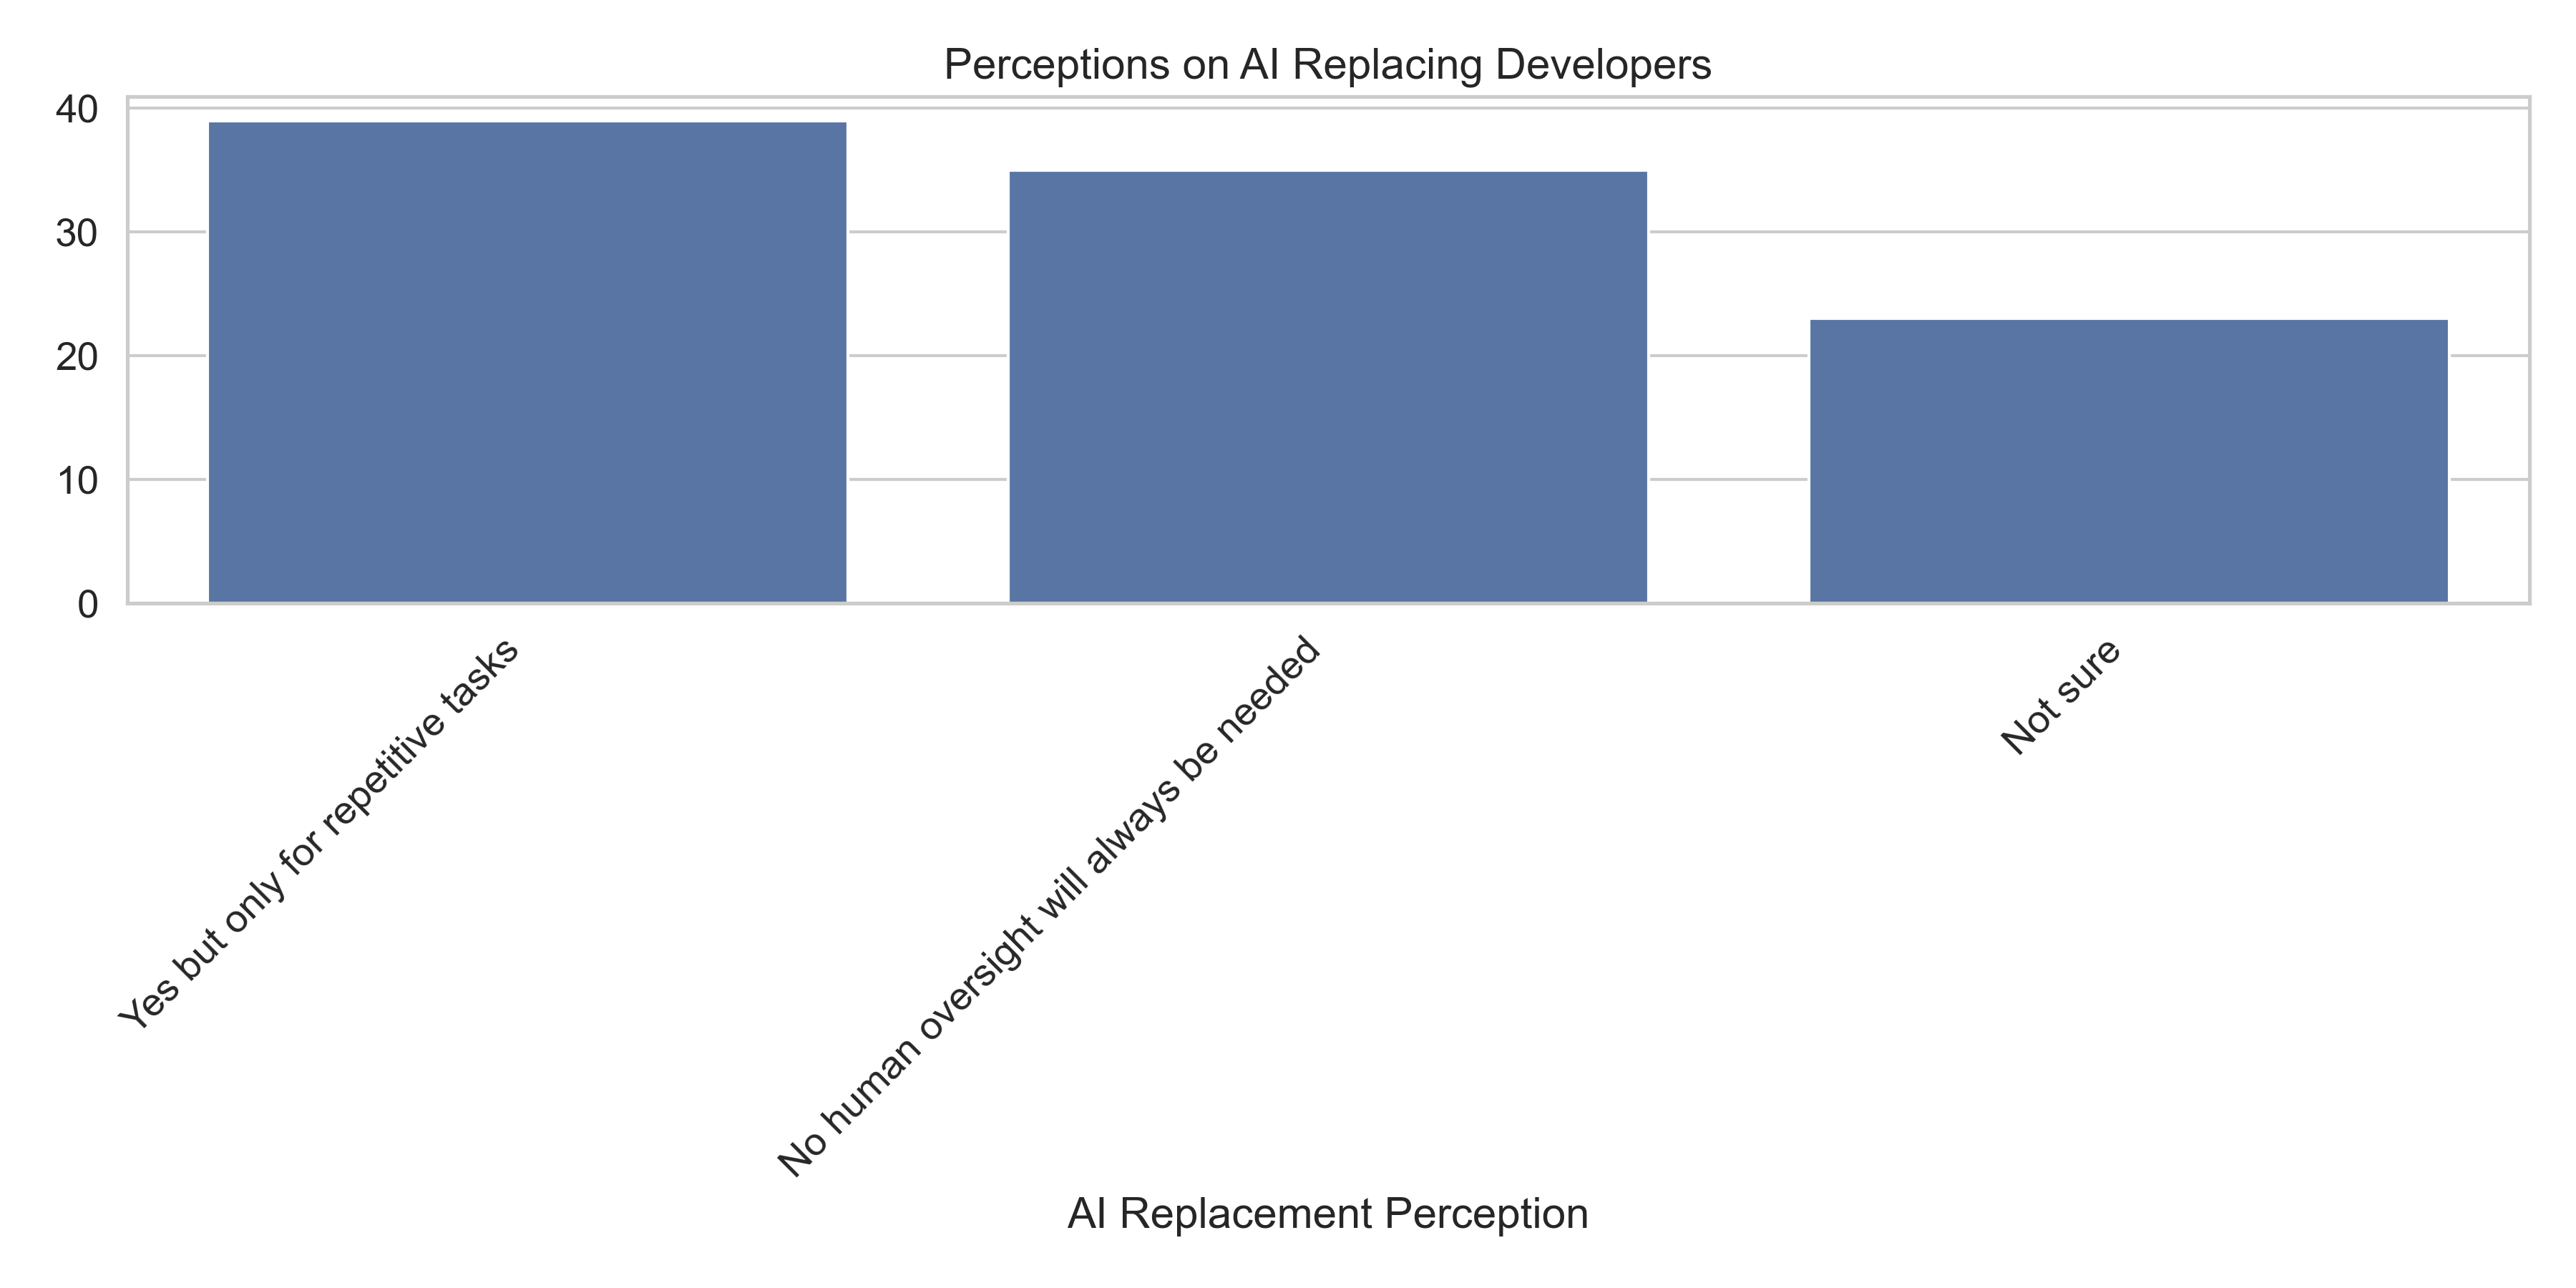
\includegraphics[width=0.8\linewidth]{final_research/replacement_perception.png}
    \caption{Perceptions on AI replacing developers}
    \label{fig:replacement_perception}
\end{figure}

This suggests that experience provides perspective on both the capabilities and limitations of AI tools in real-world development contexts.

\subsection{Implications for Tool Development}
Our findings suggest several implications for AI coding tool development:

\begin{enumerate}
    \item \textbf{Audience-specific features}: The varying concerns and usage patterns across professional roles suggest that tool developers should consider role-specific features and interfaces. For example, academic integrations with citation management for researchers or enhanced security features for freelancers.

    \item \textbf{Trust-building mechanisms}: Given the strong correlation between trust and perceived benefits, tools should incorporate transparency features that help users understand how suggestions are generated and provide quality metrics for AI-generated code.

    \item \textbf{Experience-calibrated assistance}: Tools could benefit from adapting their behavior based on user experience levels. More experienced users might appreciate automation of routine tasks while maintaining creative control, while beginners might benefit from more explanatory assistance.

    \item \textbf{Educational integration}: The high percentage of students using AI tools for learning suggests an opportunity for deeper integration with educational platforms and more explicit learning-focused features.

    \item \textbf{Addressing specific concerns}: Tools should directly address the dominant concerns of their user base, such as bias detection features for students, plagiarism checks for researchers, and security enhancements for freelancers.
\end{enumerate}

\section{Conclusion}
Our analysis demonstrates that AI coding tools are making a significant impact across the software development landscape, with adoption patterns, usage frequencies, and perceptions varying substantially across demographic and professional lines. The data reveals a nuanced picture where trust, experience, and professional context interact to shape how individuals incorporate these tools into their workflows.

The strong correlation between trust and productivity benefits suggests that AI tool effectiveness depends not only on technical capability but also on user confidence. The polarization of perceptions among experienced developers indicates that the industry is still navigating the proper role and scope of AI assistance in software development.

Professional roles emerge as a critical factor in shaping both tool usage and concerns, with each segment of the development ecosystem approaching AI tools with distinct priorities and perspectives. This finding highlights the importance of targeted, context-aware approaches to AI tool development rather than one-size-fits-all solutions.

The predominant view that AI enhances creativity rather than diminishes it suggests that these tools are finding their place as collaborative assistants rather than replacements for human creativity. This is reinforced by the finding that experienced professionals largely believe that human oversight will always be necessary, even as AI capabilities continue to advance.

As AI coding tools continue to evolve, our research suggests they will increasingly differentiate to address the specific needs, concerns, and workflows of diverse user groups across the software development ecosystem.

\section{Limitations and Future Research}
This study has several limitations that suggest directions for future research:

\textbf{Sample size and representation}: While our sample of 97 participants provided meaningful insights, a larger and more globally diverse sample would enhance generalizability. Future studies should aim for broader geographic and cultural representation.

\textbf{Longitudinal perspective}: Our cross-sectional approach captured a snapshot of current perceptions but couldn't track how attitudes toward AI tools evolve over time. Longitudinal studies would help understand how perceptions change as users gain experience with these tools.

\textbf{Objective productivity metrics}: Our reliance on self-reported productivity impacts could be supplemented in future research with objective measures of output quality and development speed.

\textbf{Specific tool comparisons}: A more granular analysis of specific tools and their features could provide greater insight into which aspects of AI assistance are most valuable across different contexts.

\textbf{Organizational context}: Future research should explore how organizational policies, team dynamics, and workplace culture influence AI tool adoption and usage patterns.

\textbf{Ethical dimensions}: Deeper investigation into the ethical implications of AI coding tools, particularly regarding bias, attribution, and intellectual property, would address important concerns highlighted in our findings.

As AI tools continue to transform software development practices, ongoing research will be essential to understand their evolving impact and guide their development in directions that maximize benefits while addressing legitimate concerns.

\section*{Acknowledgment}
The authors would like to acknowledge all survey participants who contributed their valuable perspectives to this research.

\begin{thebibliography}{00}
\bibitem{b1} A. Barke, M. Fagan, K. Aggarwal, and C. Parnin, "A Survey of Practitioners' Use of AI Tools in Software Engineering," in IEEE Transactions on Software Engineering, vol. 48, no. 9, pp. 3350-3365, 2022.

\bibitem{b2} J. Liu, Q. Huang, X. Xia, E. Shihab, D. Lo, and S. Li, "Is using deep learning frameworks free? Characterizing technical debt in deep learning frameworks," in Proceedings of the ACM/IEEE 42nd International Conference on Software Engineering, 2020, pp. 1-12.

\bibitem{b3} M. Chen, J. Tworek, H. Jun, Q. Yuan, H. P. de O. Pinto et al., "Evaluating Large Language Models Trained on Code," arXiv preprint arXiv:2107.03374, 2021.

\bibitem{b4} S. Luan, D. Yang, C. Barnaby, K. Sen, and S. Chandra, "When and How Developers Use AI Assistants: A Study of GitHub Copilot and ChatGPT," arXiv preprint arXiv:2304.06055, 2023.

\bibitem{b5} N. Peitek, S. Apel, C. Parnin, A. Brechmann and J. Siegmund, "Program Comprehension and Code Generation with Large Language Models: A Critical Examination," in IEEE Transactions on Software Engineering, vol. 49, no. 6, pp. 2602-2617, 2023.
\end{thebibliography}

\end{document} 